\documentclass[12pt,twoside,a4paper,tikz,border=5]{refart} 
% add russian language
\usepackage[utf8]{inputenc}
\usepackage[T1]{fontenc}
\usepackage[russian]{babel}

\usepackage{indentfirst}
\setlength{\parindent}{1cm}

% setup titles 
\usepackage{titlesec}
	\titleformat{\section}
		{\normalfont\fontsize{16}{0}\bfseries}{\thesection}{1em}{}
	\titleformat{\subsection}
		{\normalfont\fontsize{14}{0}\bfseries}{\thesubsection}{1em}{}
	\titleformat{\subsubsection}
		{\bf\fontsize{14}{0}}{\thesubsubsection}{1em}{}
		
	\titlespacing*{\section}
		{0pt}{5ex}{3ex} % left before after
	\titlespacing*{\subsection}
		{0pt}{3ex}{1ex}
	\titlespacing*{\subsubsection}
		{0pt}{3ex}{1ex}
	%start each section on new page
	\newcommand{\sectionbreak}{\clearpage}
	

% set up better resolution
\pdfpkmode{dpdfezzz}
\pdfpkresolution=8000

% set fraction of text
\settextfraction{0.88}

%colorbox for menu
\usepackage[most]{tcolorbox}
%\newtcbox{\menubox}{nobeforeafter,colframe=mycolor,colback=mycolor!10!white,boxrule=0.5pt,arc=4pt,
%	boxsep=0pt,left=6pt,right=6pt,top=6pt,bottom=6pt,tcbox raise base}

\definecolor{myblue}{rgb}{0.000, 1.000, 1.000}
\definecolor{dodgerblue}{rgb}{0.117,0.564,1.000}

\newtcbox{\menubox}{enhanced,nobeforeafter,tcbox raise base,boxrule=0.4pt,top=0mm,bottom=0mm,
	right=1mm,left=1mm,arc=2pt,boxsep=2pt,before upper={\vphantom{dlg}},
	colframe=blue!50!black,coltext=black,colback=myblue,
}

\robustify{\menubox}

\newtcbox{\filebox}{enhanced,nobeforeafter,tcbox raise base,boxrule=0.4pt,top=0mm,bottom=0mm,
	right=0mm,left=4mm,arc=1pt,boxsep=2pt,before upper={\vphantom{dlg}},
	colframe=green!50!black,coltext=green!25!black,colback=myblue,
	overlay={\begin{tcbclipinterior}\fill[dodgerblue] (frame.south west)
			rectangle node[text=white,font=\sffamily\bfseries\tiny,rotate=90] {FILE} ([xshift=4mm]frame.north west);\end{tcbclipinterior}}}

\robustify{\filebox}

\newtcbox{\dirbox}{enhanced,nobeforeafter,tcbox raise base,boxrule=0.4pt,top=0mm,bottom=0mm,
	right=0mm,left=4mm,arc=1pt,boxsep=2pt,before upper={\vphantom{dlg}},
	colframe=green!50!black,coltext=green!25!black,colback=myblue,
	overlay={\begin{tcbclipinterior}\fill[dodgerblue] (frame.south west)
			rectangle node[text=white,font=\sffamily\bfseries\tiny,rotate=90] {DIR} ([xshift=4mm]frame.north west);\end{tcbclipinterior}}}

\robustify{\dirbox}


% Add glosaries
\usepackage[acronym]{glossaries}
\renewcommand{\glsnamefont}[1]{\textbf{#1}}
\makeglossaries
\usepackage{enumitem} % for better alignment
\loadglsentries{glossarie.tex}

\newglossarystyle{acrostyle}{%
	\glossarystyle{long}%
	\renewenvironment{theglossary}%
	{\begin{longtable}{p{2cm}p{10cm}}}%
		{\end{longtable}}%
}

% for figures
\usepackage{subcaption}
\DeclareCaptionLabelFormat{gostfigure}{Рисунок #2}
\DeclareCaptionLabelFormat{slide}{Слайд №#2}
\DeclareCaptionLabelFormat{gosttable}{Таблица #2}
\DeclareCaptionLabelSeparator{gost}{~---~}

\captionsetup{labelsep=gost}
\captionsetup[figure]{labelformat=gostfigure}
\captionsetup[table]{labelformat=gosttable}
\captionsetup{figurewithin=none, tablewithin=none}
\renewcommand{\thesubfigure}{\asbuk{subfigure}}

%for crop
\usepackage{graphicx}



% for tables and image inside
\usepackage{array}
\usepackage{tabularx,booktabs} 
% biblio style
\bibliographystyle{utf8gost705u} 

% for margins
\setlength\oddsidemargin{-0in}
\setlength\evensidemargin{-0in}
\setlength\textwidth{165mm}

% for web links
\usepackage{hyperref}
\hypersetup{
	colorlinks=true,
	linkcolor=blue,
	urlcolor=blue,
}

\urlstyle{same}

% for header on every page
\usepackage{fancyhdr}
\usepackage{lipsum}% just to generate text for the example

\pagestyle{fancy}
\fancyhf{}
\fancyhead[L]{\rightmark}
\fancyhead[R]{\thepage}
\renewcommand{\headrulewidth}{0.4pt}
%\renewcommand{\footrulewidth}{0.4pt}% default is 0pt

% Tables and pictures captions align
\usepackage[]{caption}
\captionsetup[table]{justification=raggedleft} 
\captionsetup[figure]{justification=centering,labelsep=endash} 

% for enumerate style
\renewcommand\labelenumii{\theenumi.\arabic{enumii}.}

% for pagebreak in tabularx
\usepackage{ltablex}

% for tableitem header with italic font
%\newcounter{titem}
%\newenvironment{titem}[1][]{\refstepcounter{titem}\par\medskip
%	\textit{\thetableitem. #1} }{\medskip}




\newcounter{titem}[table]
\newenvironment{titem}[2][]{\refstepcounter{titem}\par\medskip
	\noindent \textit{
			\begin{flushleft}
				\begin{hyphenrules}{nohyphenation}
					\thetitem.~#1~#2\newline
				\end{hyphenrules}
			\end{flushleft}
			}}{\medskip}


\begin{document} 
\begin{titlepage}
	\centering
	{\scshape\small Национальный исследовательский университет \\
		``Высшая школа экономики'' \par}
	\vspace{2cm}
	{\scshape\Large ``Система интеллектуальной \\кластеризации данных'' \\
		(Intelligent Data Clustering Toolkit, INDACT)\par}
	\vspace{1.5cm}
	{\Huge\bfseries ИНСТРУКЦИЯ ПОЛЬЗОВАТЕЛЯ\par}
	\vspace{2cm}
	\vfill
	\begin{center}
		\begin{tabular}{  p{7cm}  p{4cm} p{5cm}  } 
			& & \textbf{Разработчик:}\\ 
			& & Еремейкин П.А. \\ 
			& & студент группы \\
			& & мНоД16\_ТМСС\\
			& & \\
			& & \textbf{Руководитель: }\\
			& & профессор\\
			& & Миркин Б.Г.\\
		\end{tabular}
	\end{center}
	\vfill
	{Москва \the\year\par}
\end{titlepage}

\section*{Аннотация}
Система интеллектуальной кластеризации данных представляет собой программный комплекс, предназначенный для проведения кластер-анализа с применением интеллектуальных подходов. Задача кластер-анализа состоит в разделении таблицы объектов в множества (кластеры) таким образом, чтобы сходные объекты попали в один и тот же кластер, а несходные --- в разные. Широко известен традиционный метод кластер-анализа --- \textit{k-means}. Однако, этот метод обладает существенным недостатком: для его применения необходимо знать число кластеров, на которые будут разбиты данные. Для практического применения этот недостаток зачастую вынуждает отказаться от использования \textit{k-means}. В этом случае задачу позволяют решить интеллектуальные методы, которые в процессе работы или другими способами позволяют автоматически определить число кластеров. Программная система INDACT обладает всем необходимым функционалом и включает в свой инструментарий множество методов, необходимых для решения сложных задач кластер анализа.
\newpage
	
\tableofcontents 

\newpage
\section{Введение}
\subsection{Область применения} 

Программное обеспечение ``Система Интеллектуальной Кластеризации'' (СИК) применяется для проведения кластер-анализа таблиц данных с использованием интеллектуальных алгоритмов. Типичный пример задачи для решения который может применяться кластер-анализ --- задача об ирисах Фишера. Эта задача состоит в поиске 50 экземпляров каждого из трёх видов ириса --- Ирис щетинистый (Iris setosa), Ирис виргинский (Iris virginica) и Ирис разноцветный (Iris versicolor) на данных из 150 объектов. Каждый объект обладает четырьмя признаками: 
\begin{enumerate}
	\item Длина чашелистика
	\item Ширина чашелистика
	\item Длина лепестка
	\item Ширина лепестка
\end{enumerate}
Кластер-анализ применяется во многих областях, включая компьютерное зрение, маркетинг, биоинформатику и медицину\cite{amorim}.


\subsection{Описание возможностей} 
Программа СИК предоставляет пользователю возможности просмотра таблиц данных, нормализации данных, кластер-анализа и визуализации результатов. Кроме того, возможности программы включают в себя генерацию искусственных данных. 

\subsection{Уровень подготовки пользователя}
Для работы с программой от пользователя требуется знание основ работы с графическим интерфейсом современных операционных систем (ОС).

\section{Назначение}

Система интеллектуальной кластеризации INDACT предназначена для выделения из таблиц наблюдения множеств (кластеров) таким образом, чтобы сходные объекты попадали в один и тот же кластер, а несходные — в разные кластеры \cite{data-science}. Основной целью СИК является повышение эффективности анализа данных. Функционалом системы предусмотрено два типа работ:
\begin{itemize}
	\item кластеризация реальных данных
	\item проведение численного эксперимента с синтетическими данными
\end{itemize}

\section{Условия применения}

Программный продукт работает в операционной системе Microsoft Windows 7 со следующими характеристиками:
\begin{itemize}
	\item объем ОЗУ не менее 2 Гб
	\item объем жесткого диска не менее 40 Гб
	\item микропроцессор с тактовой частотой не менее 1.5 Гц
	\item монитор с разрешением от $1280 \times 1024$ точек и выше
\end{itemize}
	Наличие дополнительного оборудования не требуется. 
	
\section{Подготовка системы к работе и запуск}
Для подготовки системы к работе требуется скопировать каталог с бинарными файлы программы с носителя на котором распространяется программа на запоминающее устройство ПК пользователя.  Каталог бинарных файлов назван \texttt{INDACT}. Для начала работы пользователь запускает на выполнение файл \texttt{INDACT.exe} из каталога бинарных файлов. 

\textbf{Внимание!} Запуск графического интерфейса может  потребовать от 10 секунд и более в зависимости от производительности ПК пользователя.\footnote{Большое время запуска графического интерфейса связано с инициализацией среды выполнения Python и загрузкой dll библиотек. В настоящее время распространение ПО для ОС Windows осуществляется при помощи утилиты \texttt{pyinstaller} (см. \url{http://www.pyinstaller.org/}), что увеличивает время запуска.} Дополнительные действия не требуются.

\section{Основные приципы работы}

\subsection{Этапы работы с программой}
Работа с программой СИК строится на основе графического диалогового интерфейса. Типичный сценарий взаимодействия пользователя с программой разделяется на следующие этапы:
\begin{enumerate}
	\item Запуск программы
	\item Загрузка исходных данных
	\item Нормализация
	\item Отбор признаков
	\item Выполнение кластеризации
	\item Просмотр результатов и текстового отчёта
\end{enumerate}

После запуска программы требуется выбрать файл, содержащий данные для кластеризации. Затем производится настройка параметров нормализации и кластеризации, а также отбор признаков, участвующих в кластеризации и выбор основных свойств применяемого алгоритма (см. \ref{subsec:norm}, \ref{subsec:gui}). После выбора необходимых параметров пользователь запускает алгоритм кластеризации. Когда выполнение кластеризации заканчивается, пользователю становятся доступны результаты работы для просмотра и анализа. 

\subsection{Требования к файлу исходных данных}
\label{subsec:req}
Источником данных для программы является текстовый файл. Следует уделить особое внимание формату файла. Ниже перечислены требования к загружаемому файлу:
\begin{enumerate}
	\item Файл содержит записи в формате таблицы
	\item Строки таблицы соответствуют объектам
	\item Столбцы таблицы соответствуют признакам
	\item Разделитель строк --- символ перевода строки (CR+LF для Windows)
	\item Разделитель столбцов --- запятая
	\item Первая строка обязательно содержит перечень названий признаков
	\item Названия признаков состоят только из латинских букв
	\item Разделитель дробной и целой части --- точка
	\item Значения номинальных признаков записываются в одно слово из латинских букв. Цифры не допустимы.
\end{enumerate}
Пример файла с  валидной структурой приведён в разделе ``\ref{subsec:trainfile} Обучающий файл''.

\subsection{Обучающий файл}
\label{subsec:trainfile}

Демонстрация возможностей программы будет проиллюстрирована на обучающем наборе данных. Файл \texttt{smartphones.dat} с демонстрационной таблицей данных можно найти в каталоге бинарных файлов программы в директории \texttt{example}. Этот файл можно открыть с помощью текстового редактора, например стандартного блокнота Windows и при необходимости отредактировать или просто посмотреть содержимое. 

Демонстрационный файл содержит таблицу параметров сматрфонов, продаваемых в магазине Ozon (\url{http://www.ozon.ru/}) в IV квартале 2017 года. Каждому смартфону соответствует 7 параметров: name, price, diag, cpu, ram, stype, vendor; соответственно название смартфона, цена в рублях, диагональ экрана в дюймах, частота процессора в ГГц, объем ОЗУ в Мб, тип матрицы, вендор.

Пример файла исходных данных, удовлетворяющий требованиям, описанным в разделе ``\ref{subsec:req} Требования к файлу исходных данных '', приведён ниже. Показаны только несколько первых строк, полный файл содержит 581 модель смартфона. Названия сокращены в целях наглядности.

\begin{tcolorbox}[colframe=black!50!black,coltext=black!25!black,colback=white,title=\textbf{Пример файла входных данных \texttt{data.csv}}]
	\verb|          name,      price,   diag,    cpu,    ram,   stype,   vendor |\\
	\verb|Meizu U10 32GB,   11990.00,    5.0,   1.50,   3072,     IPS,    Meizu |\\
	\verb|ZTE Blade A510,    7011.00,    5.0,   1.00,   1024,     IPS,      ZTE |\\
	\verb|Huawei P9 Lite,   14190.00,    5.2,   2.00,   2048,     IPS,   Huawei |\\
	\verb|Meizu M5 32GB ,   12990.00,    5.2,   1.50,   3072,     IPS,    Meizu |\\
	\verb|ZTE Blade L370,    4990.00,    5.0,   1.30,   1024,     TFT,      ZTE |\\
	\verb|BQ Aquaris M5 ,   18072.00,    5.5,   1.50,   3072,     IPS,       BQ |\\	
\end{tcolorbox}

\subsection{Нормализация}
\label{subsec:norm}
Нормализация --- это преобразование данных для приведения всех признаков к сопоставимым шкалам и началам отсчёта. Общая формула нормализации может быть записана следующим образом:

%\begin{tcolorbox}[colframe=green!50!black,coltext=green!25!black,colback=green!10!white,title=Формула нормализации]
	\begin{equation}\label{eq:normalization}
		X'=\dfrac{X-c}{r},
	\end{equation}
%\end{tcolorbox}
\noindent где $X$ --- исходные данные,\\
\phantom{где\space}$c$ --- параметр, определяющий преобразование начала отсчёта,\\
\phantom{где\space}$r$ --- параметр, определяющий преобразование масштаба шкалы.

В системе INDACT процедура нормализации реализована независимо от кластеризации и параметры нормализации могут быть изменены практически на любой стадии работы с системой. Как правило, нормализация задаётся сразу после загрузки исходных данных. Этап нормализации можно пропустить, если данные уже нормированы или в этом нет необходимости по мнению пользователя.

Выполнению кластеризации предшествует выбор параметров и принципов, на которых основывается процесс поиска однородных множеств. После выбора всех необходимых параметров пользователь производит запуск алгоритма и получает результат в интерфейсе программы. 

\subsection{Просмотр результатов кластеризации}

Просмотр результатов кластеризации может состоять в отслеживании принадлежности каждого объекта определенным кластерам или получении графического представления найденной кластерной структуры. Также система INDACT позволяет представить результат в виде интегральной таблице или в виде текстового отчёта.


\subsection{Общие сведения о пользовательском интерфейсе}

\subsubsection{Главное окно}
\label{subsec:gui}
Как было отмечено ранее, программа обладает графическим пользовательским интерфейсом. В данном разделе приведены основные сведения относительно элементов управления, их положения и функциях.


\begin{figure}[h!]
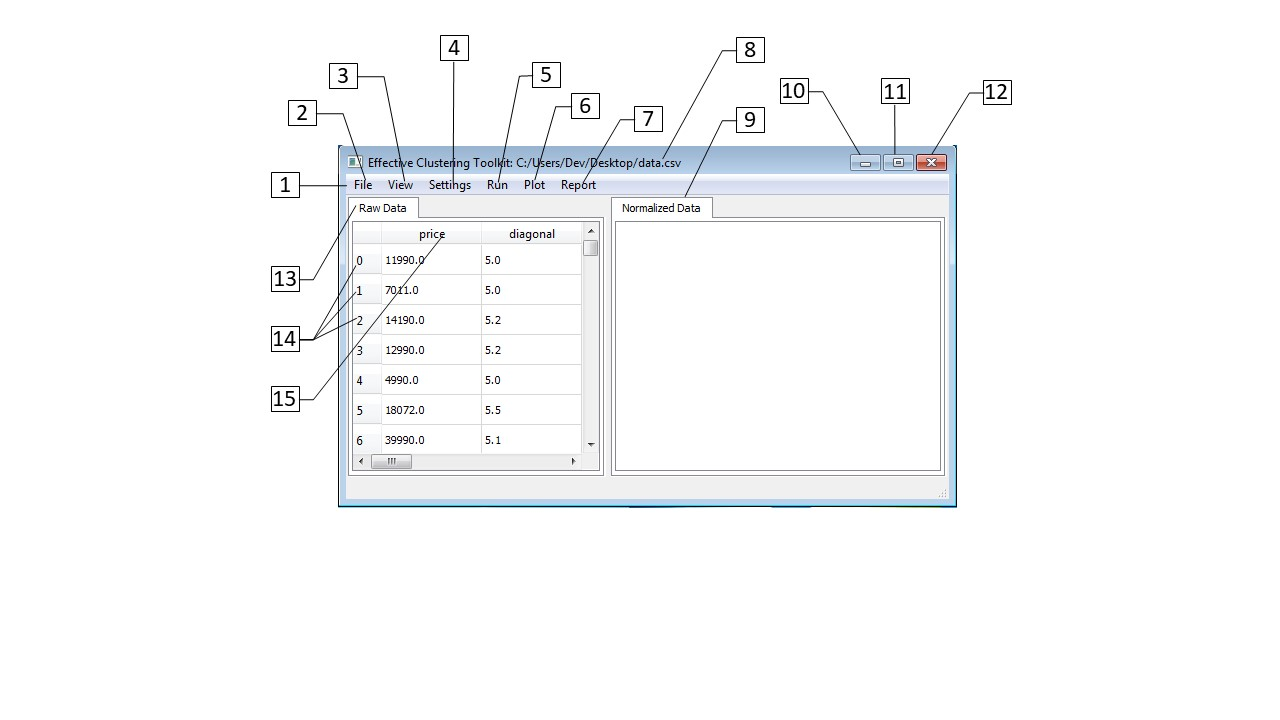
\includegraphics[trim={180 150 172  25},clip,width=0.95\textwidth]{img/guicommonannotated.jpg}
\caption{Основные элементы пользовательского интерфейса}
\label{fig:main-window}
\end{figure}
\begin{enumerate}
	\item Главное меню, элемент интерфейса, содержащий основные команды
	\item Меню File, содержит пункты:
		\begin{itemize}
			\item Open --- для загрузки файла данных
			\item Data --- для манипулирования данными
			\item Exit --- для выхода из программы
		\end{itemize}
	\item Меню View, содержит пункты:
		\begin{itemize}
			\item Layout --- для настройки способа отображения панелей данных: Tab Layout для отображения по вкладкам или Panal Layout для отбражения на двух панелях одновременно (по умолчанию, как показано на схеме) 
		\end{itemize}
	\item Меню Settings, служит для настройки параметров, содержит пункты:
		\begin{itemize}
			\item Normalization --- для задания диапазона и центра нормализации
		\end{itemize}
	\item Меню Run, содержит пункты:
		\begin{itemize}
			\item Clustering --- для настройки и запуска алгоритма кластеризации
		\end{itemize}
	\item Меню Plot, служит для вызова команд графического отображения, содержит пункты:
		\begin{itemize}
			\item Plot Data by Markers --- для построения поля рассеяния (scatter plot) по отмеченным признакам
			\item Delete All Markers --- для удаления всех отметок признаков
			\item SVD --- для построения SVD диаграммы 			
		\end{itemize}
	\item Меню Report для формирования отчёта, содержит пункты:
		\begin{itemize}
			\item Show --- для отображения отчёта 		
		\end{itemize}
	\item Заголовок окна, содержит путь к открытому файлу
	\item Вкладка с нормализованными данными 
	\item Кнопка ``Свернуть окно''
	\item Кнопка ``Развернуть окно''		
	\item Кнопка ``Закрыть окно''
	\item Вкладка с исходными данными 
	\item Номера/названия объектов
	\item Названия признаков
\end{enumerate}

\subsubsection{Контекстное меню}
В данном разделе описаны пункты контекстного меню. Контекстное меню объединяет набор действий над определенным объектом и вызывается щелчком правой кнопки мыши на этом объекте. На рисунке \ref{fig:contextmenu} показано контекстное меню для признака \texttt{price}.

\begin{figure}[t!]
	\centering
	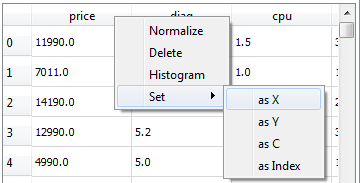
\includegraphics[width=0.45\textwidth]{img/contextmenufeature}
	\caption{Контекстное меню признака \texttt{price}}
	\label{fig:contextmenu}
\end{figure}

\newpage
Контекстное меню содержит следующие пункты:
\begin{enumerate}
	\item Normalize --- нормализует выбранный признак, добавляя его во вкладку 	``\texttt{Normalized Data}'' (см. \ref{subsubsec:onenorm})
	\item Delete --- удаляет признак из вкладки, в которой вызвано контекстное меню (см. \ref{subsubsec:deleteone})
	\item Histogram --- строит гистограмму по выбранному признаку (см. \ref{subsubsec:hist})
	\item Set --- устанавливает особые свойства для признака (см. \ref{subsubsec:scatterplot}, \ref{subsubsec:asindex})
	\begin{enumerate}
		\item as X --- выставить метку \texttt{X} для признака (см. \ref{subsubsec:scatterplot})
		\item as Y --- выставить метку \texttt{Y} для признака (см. \ref{subsubsec:scatterplot})
		\item as C --- выставить метку \texttt{C} для признака (см. \ref{subsubsec:scatterplot})
		\item as Index --- установить признак как индекс (см. \ref{subsubsec:asindex})
	\end{enumerate}
\end{enumerate}

\subsubsection{Диалог нормализации}

На рисунке \ref{fig:normdialog} показан диалог нормализации. Это окно требует от пользователя выставить значения для проведения нормализации (см. \ref{sec:norm}). 

\begin{figure}[h!]
	\centering
	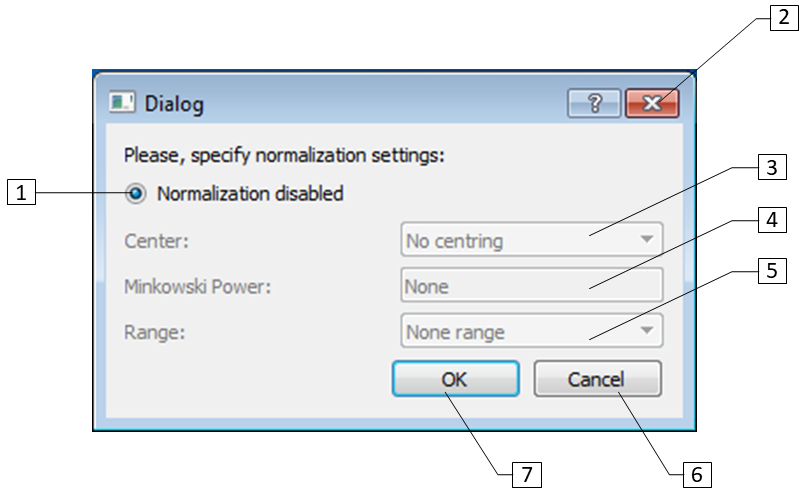
\includegraphics[width=0.55\textwidth]{img/normdialog}
	\caption{Диалог установки параметров нормализации}
	\label{fig:normdialog}
\end{figure}

\begin{enumerate}
	\item Переключатель вкл./выкл. нормализацию
	\item Кнопка закрытия окна
	\item Выпадающий список для выбора центра нормализации
	\item Поле ввода степени Минковского (активно когда выбран центр Минковского)
	\item Выпадающий список для выбора диапазона нормализации
	\item Кнопка подтверждения ввода
	\item Кнопка отмены
\end{enumerate}

\subsubsection{Окно графической информации}

Окно графической информации служит для просмотра различного вида графиков и диаграмм. Такое окно может встретиться пользователю, например при построении гистограммы (раздел \ref{subsubsec:hist}), SVD диаграммы (\ref{subsubsec:svd}) или поля рассеяния (\ref{subsubsec:scatterplot}).

\begin{figure}[h!]
	\centering
	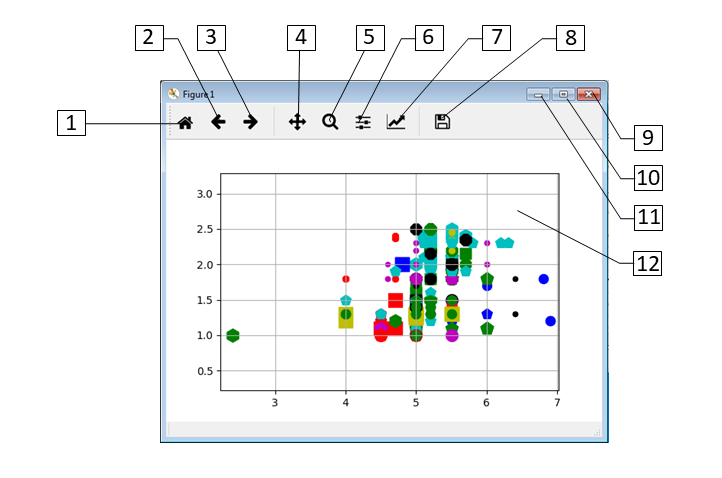
\includegraphics[width=0.9\textwidth]{img/plotview}
	\caption{Окно графической информации}
	\label{fig:plottview}
\end{figure}

\begin{enumerate}
	\item Кнопка восстановления исходного автоматического положения и масштаба
	\item Кнопка возврата к предыдущему виду (после масштабирования или смещения)
	\item Кнопка возврата к следующему виду (после масштабирования или смещения)
	\item Кнопка смещения диаграммы
	\item Кнопка масштабирования выбранной области
	\item Кнопка конфигурации отображения
	\item Кнопка редактирования осей
	\item Кнопка сохранения текущего графика в файл
\end{enumerate}

\subsubsection{Окно генерации данных}

Окно генерации применяется при работе с синтетическими данными (см. раздел \ref{subsec:generation}). Это окно необходимо для ввода информации о значениях характеристик генерируемых данных.

\begin{figure}[h!]
	\centering
	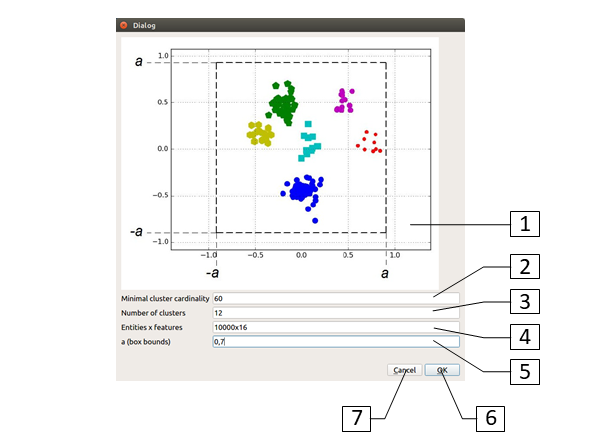
\includegraphics[width=0.9\textwidth]{img/generationwindow}
	\caption{Окно генерации данных}
	\label{fig:generationwindow}
\end{figure}

\begin{enumerate}
	\item Графическая иллюстрация смысла параметра \textit{a}
	\item Поле ввода минимального числа объектов в каждом кластере
	\item Поле ввода числа кластеров
	\item Поле ввода размерности данных (число объектов \texttt{x} число признаков)
	\item Поле ввода параметра \textit{a}
	\item Кнока подтверждения ввода
	\item Кнопка отмены ввода
\end{enumerate}



\subsubsection{Окно запуска кластеризации}

Для запуска кластеризации от пользователя требуется выставить ряд параметров в соответствии со значениями которых после будет автоматически выбран подходящий алгоритм кластеризации. На рисунке \ref{fig:runclusteringwindow} показано окно для ввода этих параметров.

\begin{figure}[h!]
	\centering
	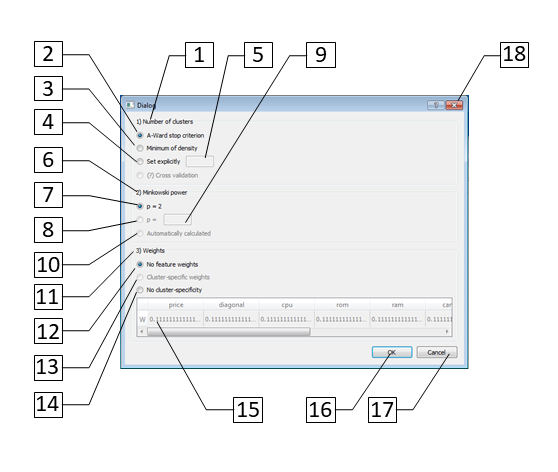
\includegraphics[width=0.9\textwidth]{img/runclusteringwindow}
	\caption{Окно запуска кластеризации}
	\label{fig:runclusteringwindow}
\end{figure}


\begin{enumerate}
	\item Группа опций, отвечающая за число кластеров
	\item Переключатель определения числа кластеров по критерию A-Ward (подробнее см. \cite{mirkin_formula_8})
	\item Переключатель поиска числа кластеров в процессе кластеризации по принципу минимума функции плотности \cite{kovaleva}
	\item Переключатель явного задание числа кластеров 
	\item Поле ввода для явного задания числа кластеров 
	\item Группа опций для установки степени Минковского (см. \cite{amorim})
	\item Переключатель, задающий степень Минковского равной 2
	\item Переключатель явного ввода степени Минковского с клавиатуры
	\item Поле ввода для степени Минковского
	\item Автоматически вычисляемая степень Минковского (в будующих версиях)
	\item Группа опций, определяющих веса признаков
	\item Переключатель отключающий веса признаков
	\item Переключатель включающий индивидуальные веса для каждого признака (см. \cite{amorim}, $A-Ward_{p\beta}$)
	\item Переключатель включающий одинаковые веса в пределах всех данных, но задаваемых для каждого признака индивидуально 
	\item Таблица для ввода весов признаков
	\item Кнопка подтверждения ввода
	\item Кнопка отмены
	\item Кнопка закрытия окна
\end{enumerate}



\subsubsection{Окно таблицы результатов}

Окно таблицы результатов служит для интегрального представления полученной кластерной структуры. Это окно может быть вызвано после выполнения шага кластеризации (см. \ref{subsec:report}). Значение таблиы соответствует среднему значению данного признака в данном кластере. Если это значение существенно больше общего среднего по признаку, то ячейка выделяется красным цветом, если существенно меньше --- синим.

\begin{figure}[h!]
	\centering
	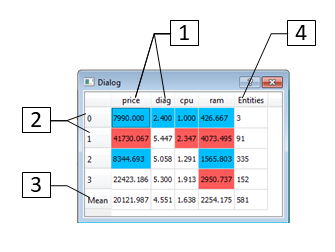
\includegraphics[width=0.55\textwidth]{img/tableresultwindow}
	\caption{Окно таблицы результатов}
	\label{fig:tableresultwindow}
\end{figure}

\begin{enumerate}
	\item Название признаков
	\item Номера кластеров
	\item Строка средних значений по всем данным
	\item Столбец числа объектов в кластере
\end{enumerate}



\newpage
\section{Описание операций}


\subsection{Запуск программы}
Для работы с программой требуется запустить процесс OC, который отображает графический интерфейс и взаимодействует с пользователем. Действия этой операции приведены в таблице ниже.

\noindent\begin{tabularx}{\textwidth}{p{5.1cm}X}
	\toprule
	\textbf{Действие/Описание}& \textbf{Интерфейс}  \\
	
	\midrule
	\begin{titem}{Запустить бинарный файл программы}
		Дважды нажать левой кнопкой мыши (ЛКМ) на значке \texttt{INDACT.exe} 
	\end{titem}
	&  \raisebox{-\totalheight}{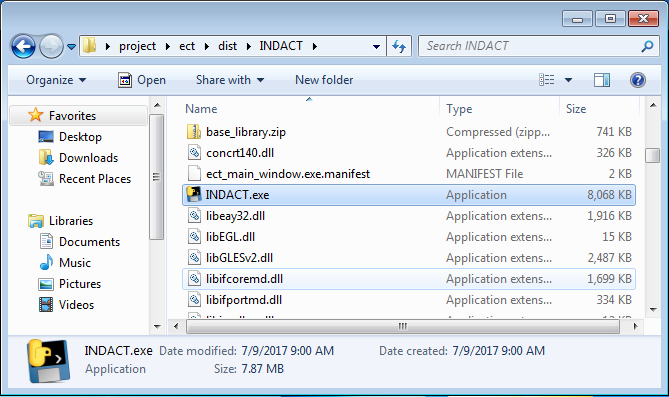
\includegraphics[width=0.65\textwidth]{img/runexe}} \\
	
	\midrule
	\begin{titem}{Дождаться запуска}
		Подождать, пока произойдёт инициализация среды выполнения Python. Открытие чёрного консольного окна, означает что установлена отладочная версия программы. Его не следует закрывать.   
	\end{titem}
	&  \raisebox{-\totalheight}{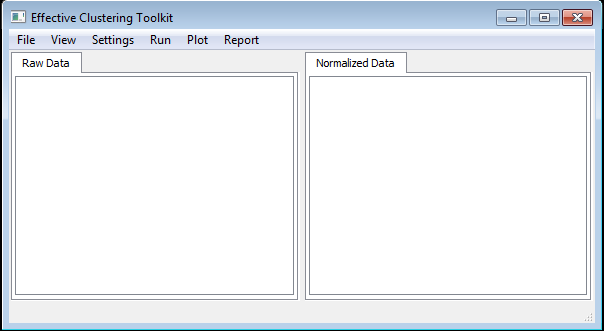
\includegraphics[width=0.65\textwidth]{img/gui}} \\
		
	\bottomrule
\end{tabularx}	

\newpage
\subsection{Загрузка исходных данных}
\label{subsec:dataload}

Загрузка данных необходима для того чтобы подать программе файл, который содержит таблицу данных. Формат файла должен удовлетворять набору требований, перечисленных в разделе ``\ref{subsec:req} Требования к файлу исходных данных''. 

\noindent\begin{tabularx}{\textwidth}{p{5.1cm}X}
	\toprule
	\textbf{Действие/Описание}& \textbf{Интерфейс}  \\
	
	\midrule
	\begin{titem}{Открыть диалог загрузки файла}
			Для открытия диалога загрузки файла необходимо последовательно нажать в главном меню пункты \menubox{\texttt{File}} $ \Rightarrow $ \menubox{\texttt{Open}}. 
	\end{titem}
	&  \raisebox{-\totalheight}{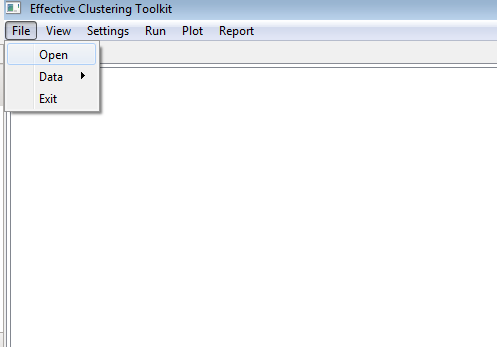
\includegraphics[trim={0 200 172 0 0},clip,width=0.65\textwidth]{img/fileopen}}	\\

	\midrule
	\begin{titem}{Выбрать текстовый файл с данными}
			В файловом диалоге необходимо выбрать загружаемый файл и нажать кнопку \menubox{\texttt{Open}}. Например, для загрузки демонстрационного примера следует выбрать файл \texttt{INDACT/example/} \texttt{smartphones.dat} 
	\end{titem}
	&  \raisebox{-\totalheight}{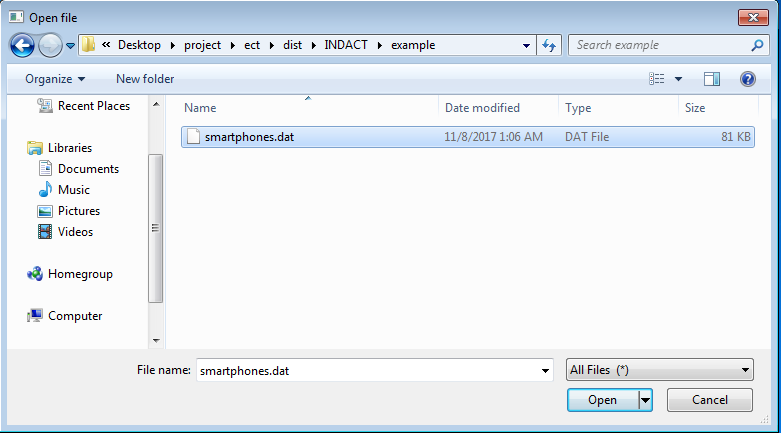
\includegraphics[width=0.65\textwidth]{img/filedialog.png}} \\	

	\midrule
	\begin{titem}{Проверить загрузку исходного файла}
		После выполнения предыдущего пункта будет произведена загрузка файла и отображение его содержимого в виде таблицы в интерфейсе программы. Пользователю следует убедиться, что загружен правильный файл, объекты и признаки отображаются верно. На рисунке справа показан загруженный файл \texttt{smartphones.dat} 
	\end{titem}
	&  \raisebox{-\totalheight}{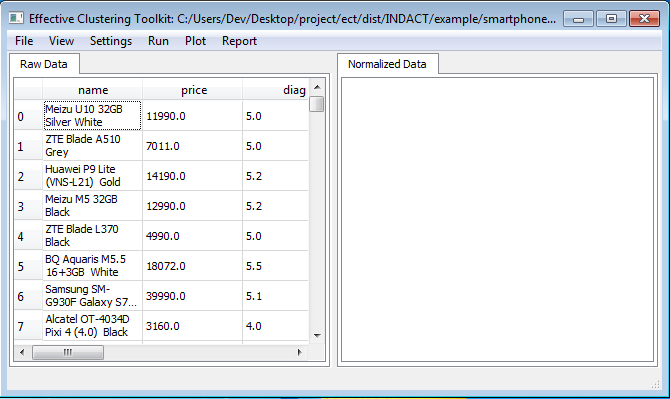
\includegraphics[width=0.65\textwidth]{img/loadeddata.png}}	\\
	\bottomrule
\end{tabularx}	

\subsection{Нормализация}
\label{sec:norm}
\subsubsection{Установка параметров нормализации}

Назначение и параметры нормализации описаны в разделе ``\ref{subsec:norm} Нормализация''.

\noindent\begin{tabularx}{\textwidth}{p{5.1cm}X}
	\toprule
	\textbf{Действие/Описание}& \textbf{Интерфейс}  \\
	\midrule
	\begin{titem}{Открыть диалог нормализации}
		Диалог нормализации можно открыть выбрав в главном меню пункты \menubox{\texttt{Settings}} $ \Rightarrow $ \menubox{\texttt{Normalization}}.
	\end{titem}
	&  \raisebox{-\totalheight}{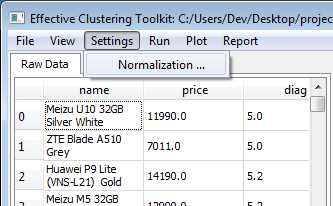
\includegraphics[trim={0 50 0 0},clip,width=0.65\textwidth]{img/opennormalizationdialog.png}}\\
	
	\midrule
	\begin{titem}{Включить нормализацию}
		Чтобы включить нормализацию требуется снять отметку с пункта ``\texttt{Normalization disabled}''. Выполнение этого действия снимет блокировку с полей параметров нормализации.
	\end{titem}
	&  \raisebox{-\totalheight}{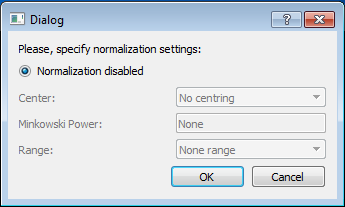
\includegraphics[width=0.65\textwidth]{img/normalizationdialog.png}} \\

	\midrule
	\begin{titem}{Выставить параметры}
		Для нормализации данных необходимо задать центр и диапазон нормализации. Эти параметры выбираются из выпадающих списков. Для завершения настройки нормализации нажать кнопку \menubox{\texttt{OK}}. Пример установки параметров приведён в разделе \ref{subsubseq:example_norm1}. 
	\end{titem}
	&  \raisebox{-\totalheight}{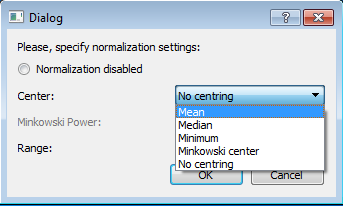
\includegraphics[width=0.65\textwidth]{img/normalizationenableddialog.png}} \\
	\bottomrule
\end{tabularx}

\newpage
\subsubsection{Нормализация одного признака}
\label{subsubsec:onenorm}
После настройки параметров нормализации необходимо выбрать какие признаки требуется нормализовать. Только выбранные признаки будут участвовать в кластеризации. В программе предусмотрено три возможности для выбора признаков: выбор по одному, выбор всех сразу и удаление по одному. 

\noindent\begin{tabularx}{\textwidth}{p{5.1cm}X}
	\toprule
	\textbf{Действие/Описание}& \textbf{Интерфейс}  \\
	\midrule
	
	\begin{titem}{Выбрать признак для нормализации}
		Для выбора одного признака необходимо найти столбец признака во вкладке ``\texttt{Raw Data}'' и нажать на нем правой кнопкой мыши (ПКМ). В контекстном меню выбрать пункт \menubox{\texttt{Normalize}}. На примере показана операция нормализации признака \texttt{stype}.
	\end{titem}
	&  \raisebox{-\totalheight}
	{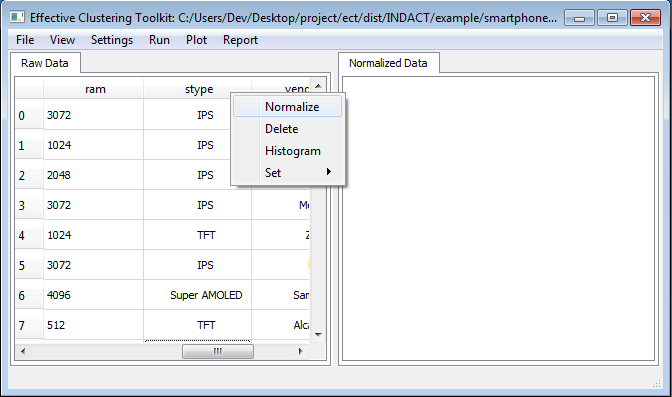
\includegraphics[trim={0 0 0 0},clip,width=0.65\textwidth]{img/normalizeonefeature.png}}
	\\
	
	\midrule
	\begin{titem}{(При необходимости) Подтвердить нормализацию категориального признака}
			Если был выбран категориальный признак (в примере \texttt{stype}), то программа запросит подтверждение разложения признака на бинарные. В случае согласия произойдёт добавление бинарных признаков, отвечающих за наличие каждого из значений категориального признака \textit{ и их нормализация}.
	\end{titem}
	 &  \raisebox{-\totalheight}{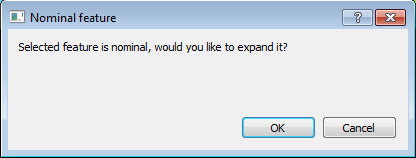
\includegraphics[width=0.65\textwidth]{img/approvenominal.png}} \\

	\midrule
	\begin{titem}{Просмотр вида таблицы}
			После выбора признака, он будет перенесён из вкладки ``\texttt{Raw Data}'' во вкладку ``\texttt{Normalized Data}'' и к нему будут применены выбранные настройки нормализации. Дополнительно во вкладке  ``\texttt{Normalized Data}'' будет отображён столбец ``\texttt{Cluster\#}'', который будет оставаться заполненным символами ``\texttt{?}'' до тех пор, пока не будет выполнен шаг кластеризации (см. верхний рисунок, нормализация признака \texttt{price}). Сказанное выше справедливо и для номинального признака (например \texttt{stype}), но стоит иметь ввиду что соответствующие бинарные признаки будут названы \texttt{stype[значение признака]} (как показано на нижнем рисунке)
	\end{titem}
	 &  \raisebox{-\totalheight}{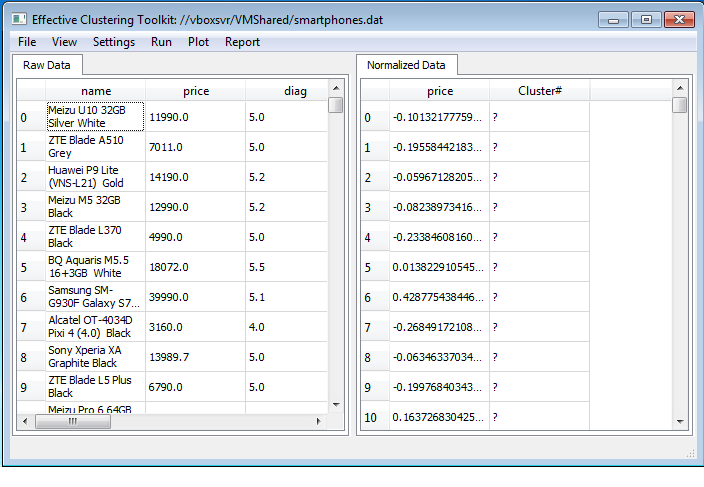
\includegraphics[width=0.65\textwidth]{img/normalizedonefeature.png}} 

		 \raisebox{-\totalheight}{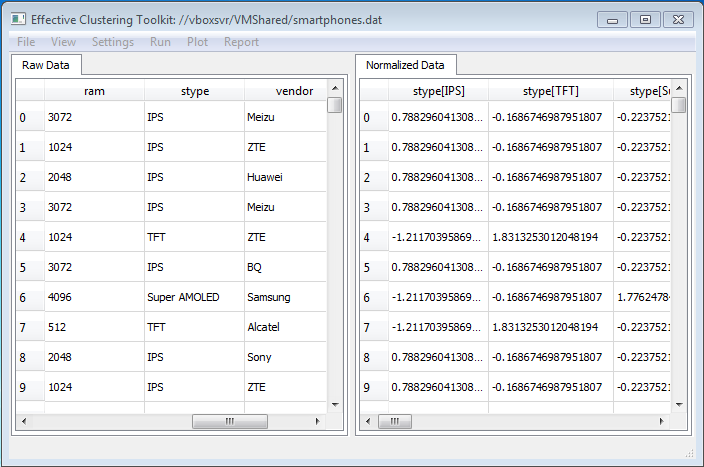
\includegraphics[width=0.65\textwidth]{img/normalizedonenominalfeature.png}}	\\
	\bottomrule
\end{tabularx}

\newpage
\subsubsection{Нормализация всех признаков сразу}

Если признаков много и нормализовать их по одному долго, то можно воспользоваться функцией нормализации всех признаков сразу.

\noindent\begin{tabularx}{\textwidth}{p{5.1cm}X}
	\toprule
	\textbf{Действие/Описание}& \textbf{Интерфейс}  \\
	\midrule
	\begin{titem}{Запустить нормализацию всех признаков }
			Для запуска нормализации всех признаков сразу, требуется в главном меню выбрать \menubox{\texttt{File}} $ \Rightarrow $ \menubox{\texttt{Data}}  $ \Rightarrow $  \menubox{\texttt{Normalize All}}.
	\end{titem}
	&  \raisebox{-\totalheight}{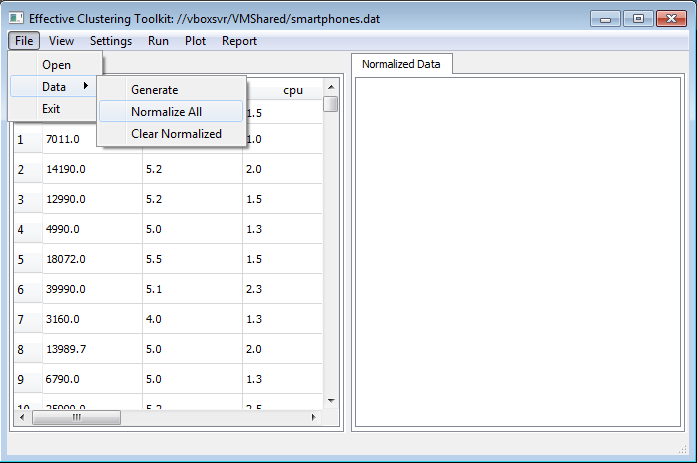
\includegraphics[width=0.65\textwidth]{img/normalizeall.png}} \\
	
	\midrule
	\begin{titem}{(При необходимости) Подтвердить нормализацию категориального признака}
		Если имеется хотя бы один категориальный признак, то программа запросит подтверждение разложения признака по количеству уникальных значений. В случае согласия программа представит номинальный признак с помощью бинарных.
	\end{titem}
	&  \raisebox{-\totalheight}{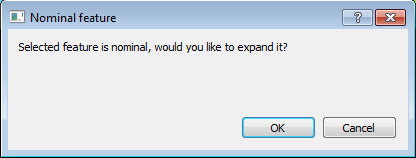
\includegraphics[width=0.65\textwidth]{img/approvenominal.png}}	\\

	\midrule
	\begin{titem}{Посмотреть результат}	
		После нормализации признаков результат будет отображен во вкладке ``\texttt{Normalized Data}''
	\end{titem}
	&  \raisebox{-\totalheight}{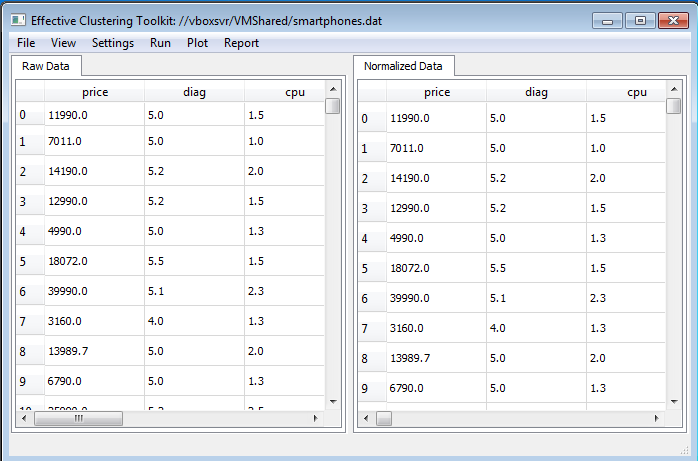
\includegraphics[width=0.65\textwidth]{img/normalizeallresult.png}}	\\
	\bottomrule
\end{tabularx}


\newpage
\subsection{Отбор признаков}
\subsubsection{Удаление одного признака}
\label{subsubsec:deleteone}

Как было отмечено выше, программа позволяет удалять отдельные признаки из как вкладки ``\texttt{Normalized Data}'' так и ``\texttt{Raw Data}''. Эта функция может быть применена для исключения из рассмотрения определённых признаков.

\noindent\begin{tabularx}{\textwidth}{p{5.1cm}X}
	\toprule
	\textbf{Действие/Описание}& \textbf{Интерфейс}  \\

	\midrule
	\begin{titem}{Выбрать признак \\ для удаления}	
	Для удаления одного признака необходимо найти столбец признака в нужной вкладке и нажать на нём ПКМ. В контекстном меню выбрать пункт \menubox{\texttt{Delete}}. 
	
	Рассмотрим удаление на примере признака \texttt{diag}. Контекстное меню, открытое после нажатия на заголовке \texttt{diag} показано на рисунке справа.
	\end{titem}
	&  \raisebox{-\totalheight}{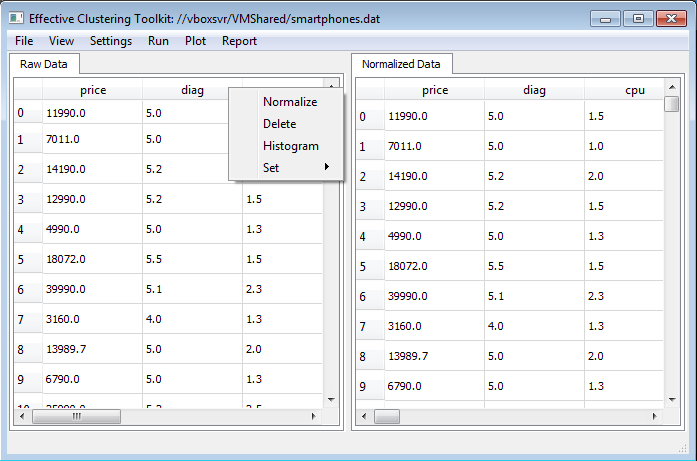
\includegraphics[width=0.65\textwidth]{img/deleteone}}	\\

	\midrule
	\begin{titem}{Посмотреть результат}
		В результате выполнения операции выбранный признак будет удалён только из вкладки ``\texttt{Raw Data}'', но останется во второй вкладке.
	\end{titem}
	&  \raisebox{-\totalheight}{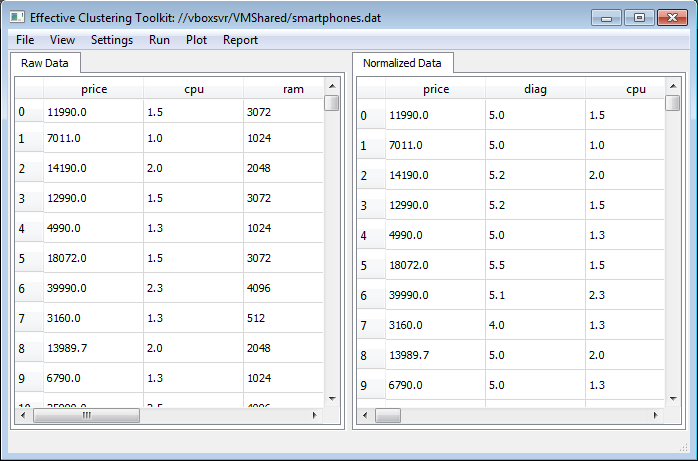
\includegraphics[width=0.65\textwidth]{img/deleteoneresult}} \\
	\bottomrule
\end{tabularx}

\newpage
\subsubsection{Удаление всех признаков сразу}

Если требуется полностью очистить вкладку ``\texttt{Normalized Data}'', то следует воспользоваться функцией, описанной ниже. Функция очистки вкладки нормализованных данных применяется для того чтобы сбросить выбор всех признаков.

\noindent\begin{tabularx}{\textwidth}{p{5.1cm}X}
	\toprule
	\textbf{Действие/Описание}& \textbf{Интерфейс}  \\

	\midrule
	\begin{titem}{Запустить удаление}
		Функция удаления всех признаков сразу вызывается из главного меню программы: \menubox{\texttt{File}} $ \Rightarrow $ \menubox{\texttt{Data}}  $ \Rightarrow $  \menubox{\texttt{Clear Normalized }}
	\end{titem}
	&  \raisebox{-\totalheight}{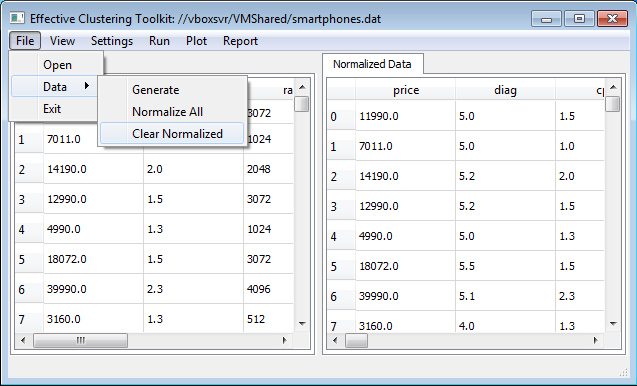
\includegraphics[width=0.65\textwidth]{img/clearnormalized}} \\

	\midrule
	\begin{titem}{Посмотреть результат}	
		В результате выполнения операции вкладка ``\texttt{Normalized Data}'' будет очищена полностью.
	\end{titem}
	&  \raisebox{-\totalheight}{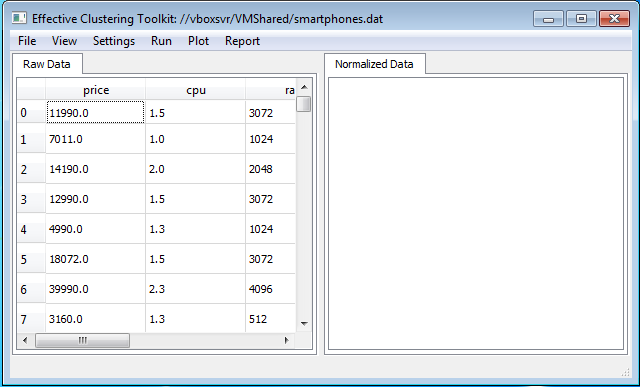
\includegraphics[width=0.65\textwidth]{img/clearnormalizedresult}} \\

	\bottomrule	
\end{tabularx}



\subsubsection{Установка признака как индекс}
\label{subsubsec:asindex}

Допустим, исходный файл содержит признак, который не требуется использовать для анализа, но который был бы полезен как уникальный индекс, например, это может быть название модели телефона. В таком случае в программе предусмотрена функция задания признака в качестве индекса. 

\newpage

\noindent\begin{tabularx}{\textwidth}{p{5.1cm}X}
	\toprule
	\textbf{Действие/Описание}& \textbf{Интерфейс}  \\
	
	\midrule
	\begin{titem}{Загрузить файл}
		Загрузка файла описана в разделе ``\ref{subsec:dataload} Загрузка исходных данных''.
	\end{titem}
	&  \raisebox{-\totalheight}{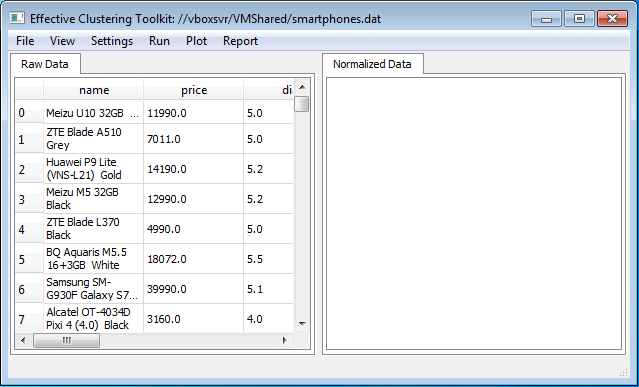
\includegraphics[width=0.65\textwidth]{img/loadnamed}} \\
	
	\midrule
	\begin{titem}{Выбрать признак}
		Для выбора признака необходимо найти его столбец в одной из вкладок и нажать ПКМ на нём. В контекстном меню выбрать пункт \menubox{\texttt{Set}} $\Rightarrow$ \menubox{\texttt{As Index}} 
	\end{titem}
	&  \raisebox{-\totalheight}{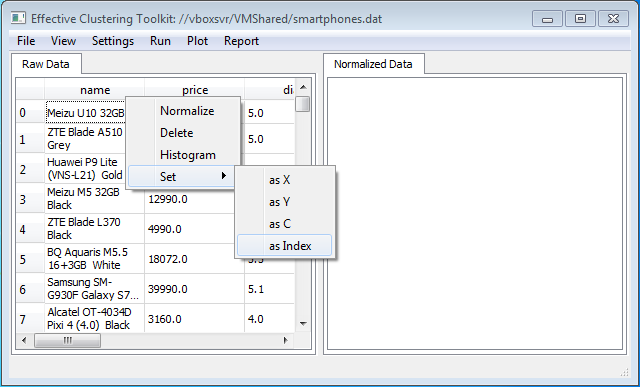
\includegraphics[width=0.65\textwidth]{img/asindex}} \\
	
	\midrule
	\begin{titem}{Посмотреть результат}
		Результат выполнения предыдущего действия состоит в отображении признака в колонке индекса как показано на рисунке справа.
	\end{titem}
	&  \raisebox{-\totalheight}{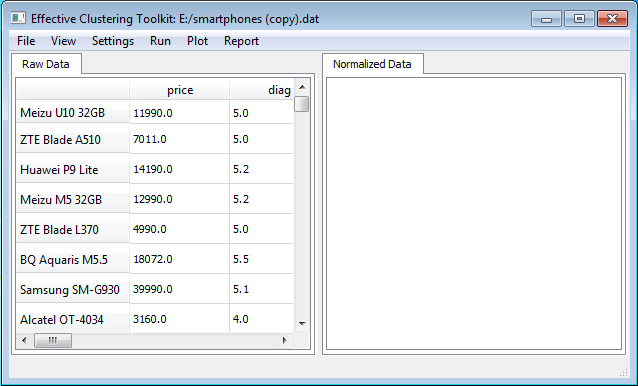
\includegraphics[width=0.65\textwidth]{img/asindexcompleted}} \\
	\bottomrule
\end{tabularx}

\newpage
\subsection{Настройка способа отображения вкладок}

Программа имеет два способа отображения данных: с помощью вкладок и с помощью панелей (по умолчанию).Для переключения этих способов служит пункт меню \menubox{\texttt{View}}

\noindent\begin{tabularx}{\textwidth}{p{5.1cm}X}
	\toprule
	\textbf{Действие/Описание}& \textbf{Интерфейс}  \\
	
	\midrule
	\begin{titem}{Переключить способ отображения}
		Для переключения способа отображения следует выбрать из главного меню программы: \menubox{\texttt{View}} $ \Rightarrow $ \menubox{\texttt{Layout}}  $ \Rightarrow $  \menubox{\texttt{Tab Layout}} или \menubox{\texttt{Panel Layout}}
	\end{titem}
	&  \raisebox{-\totalheight}{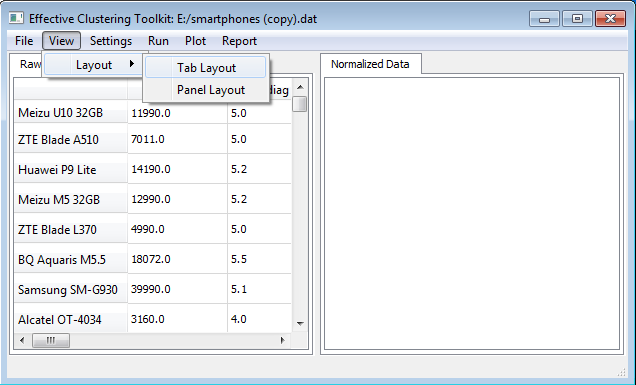
\includegraphics[width=0.65\textwidth]{img/view1}} \\

	\midrule
	\begin{titem}{Посмотреть результат}
	В результате выполнения операции панели ``\texttt{Raw Data}'' и ``\texttt{Normalized Data}'' будут отображены одна за другой.
	\end{titem}
	&  \raisebox{-\totalheight}{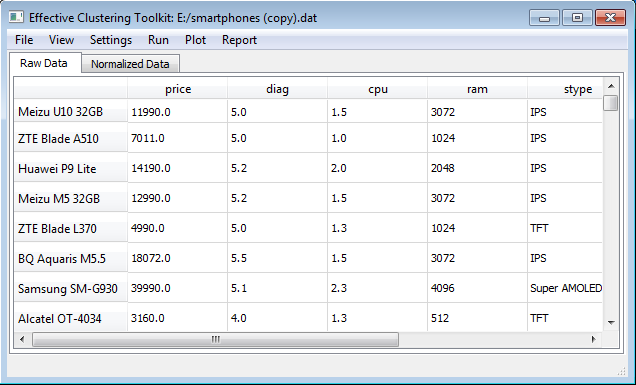
\includegraphics[width=0.65\textwidth]{img/tabview}} \\
	
	\bottomrule
\end{tabularx}

\newpage
\subsection{Визуализация}
\subsubsection{Построение гистограммы по признаку }
\label{subsubsec:hist}

В качестве первичного инструмента анализа программа предлагает возможность построения гистограммы по выбранному признаку.

\noindent\begin{tabularx}{\textwidth}{p{5.1cm}X}
	\toprule
	\textbf{Действие/Описание}& \textbf{Интерфейс}  \\

	\midrule
	\begin{titem}{Выбрать признак}
		Для выбора признака необходимо найти его столбец в одной из вкладок и нажать ПКМ на нём. В контекстном меню выбрать пункт \menubox{\texttt{Histogram}}. На примере показано построение гистограммы по признаку \texttt{price}.
	\end{titem}
	&  \raisebox{-\totalheight}{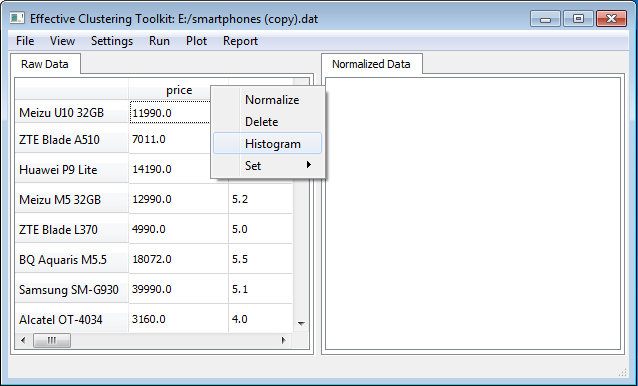
\includegraphics[width=0.65\textwidth]{img/histmenu}} \\
	
	\midrule
	\begin{titem}{Посмотреть результат}
		После выбора признака будет построена гистограмма в отдельном окне. 
	\end{titem}
	&  \raisebox{-\totalheight}{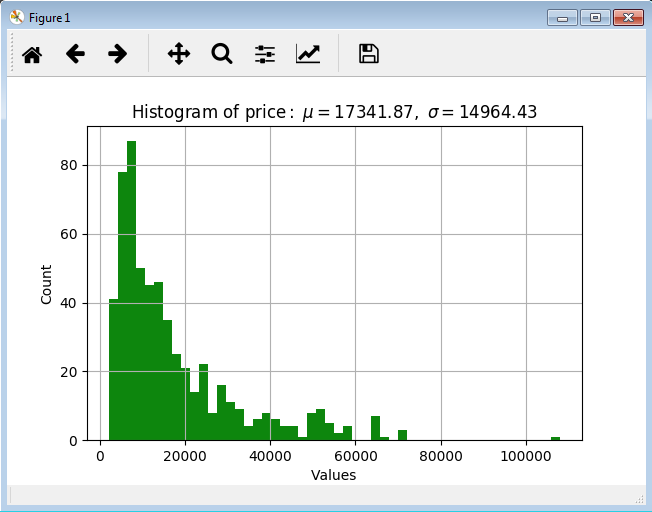
\includegraphics[width=0.65\textwidth]{img/histexample}} \\
	\bottomrule
\end{tabularx}

\newpage
\subsubsection{Построение поля рассеяния (scatter plot)}
\label{subsubsec:scatterplot}

Для первичного анализа структуры данных или результатов кластеризации в программе предусмотрена функция построения поля рассеяния по меткам на выбранных признаках. Метка --- вспомогательный символ, присваиваемый пользователем для  определённого признака.  Предусмотрено 3 вида меток: ``\texttt{X}'', ``\texttt{Y}'', ``\texttt{C}''. Первый вид означает что отмеченный признак будет соответствовать координатам объекта по оси абсцисс, второй --- по оси ординат, а третий, что цвет (\textit{Color}) точки будет выбираться в соответствии со значением отмеченного признака

\noindent\begin{tabularx}{\textwidth}{p{5.1cm}X}
	\toprule
	\textbf{Действие/Описание}& \textbf{Интерфейс}  \\
	
	\midrule
	\begin{titem}{Выбрать признак по оси X}
		Для построения поля рассеяния требуется задать признаки по осям абсцисс и ординат. Чтобы отметить признак, соответствующий оси абсцисс, требуется нажать на его названии ПКМ и в контекстном меню выбрать
		\menubox{\texttt{Set}} $\Rightarrow$ \menubox{\texttt{as X}} 
	\end{titem}
	&  \raisebox{-\totalheight}{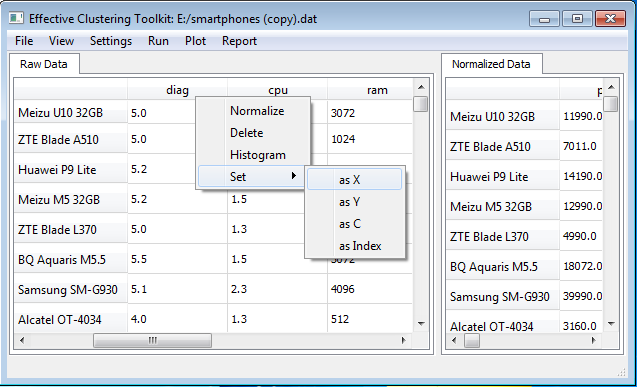
\includegraphics[width=0.65\textwidth]{img/setasx}} \\
	
	\midrule
	\begin{titem}{Посмотреть результат}
			После установки маркера ``\texttt{X}'' к имени соответствующего признак добавиться ``\texttt{(X)}''
	\end{titem}
	&  \raisebox{-\totalheight}{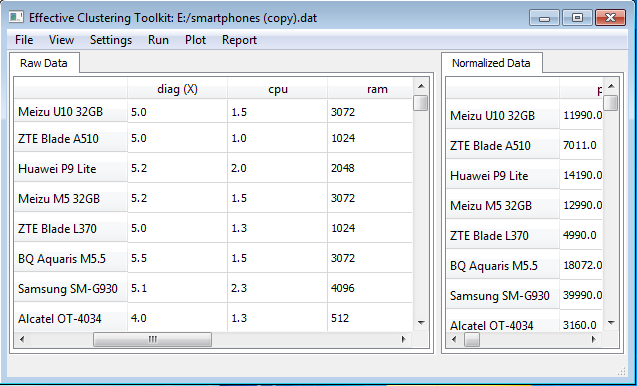
\includegraphics[width=0.65\textwidth]{img/setasxresult}} \\	
	
	\midrule
	\begin{titem}{Выбрать признак по оси Y}
	\end{titem}
	& 	\parbox[t]{12cm}{ \vphantom{нечто} Аналогично пунктам 1,2.} \\
	
	\midrule
	\begin{titem}{Выбрать признак отвечающий за цвет точек}
		Для того чтобы задать какой признак будет определять цвет точек на диаграмме необходимо выставить маркер \texttt{C}. Для этого выбрать признак, нажать ПКМ и в контекстном меню выбрать \menubox{\texttt{Set}} $\Rightarrow$ \menubox{\texttt{as С}} 
	\end{titem}
	&  \raisebox{-\totalheight}{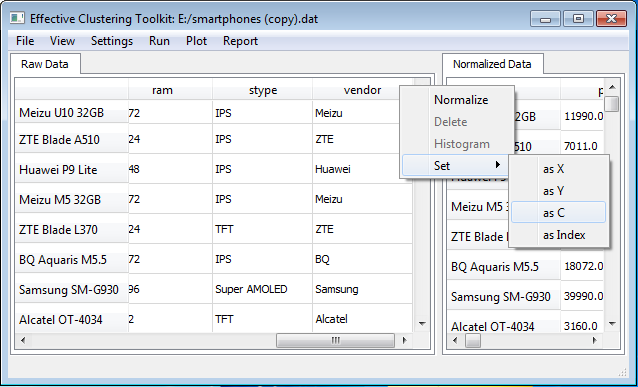
\includegraphics[width=0.65\textwidth]{img/setcmarker}} \\
	
	\midrule
	\begin{titem}{Построить sctter plot}
		В главном меню выбрать \menubox{\texttt{Plot}} $\Rightarrow$ \menubox{\texttt{Plot Data by Markers}} 
	\end{titem}
	&  \raisebox{-\totalheight}{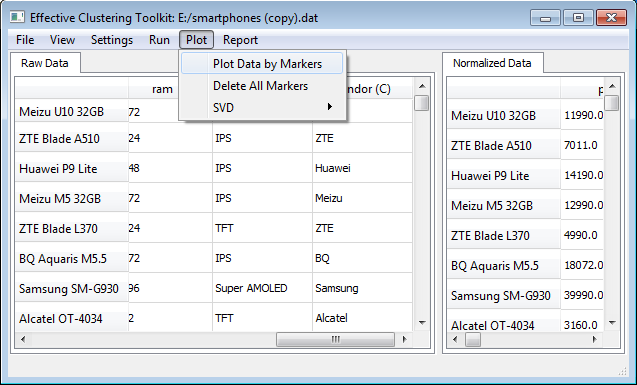
\includegraphics[width=0.65\textwidth]{img/plotbymarkers}}\\
	
	\midrule
	\begin{titem}{Посмотреть результат}
			В новом окне откроется построенная диаграмма
	\end{titem}
	&  \raisebox{-\totalheight}{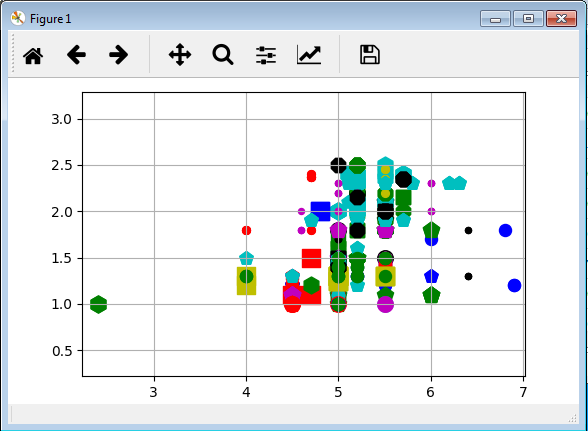
\includegraphics[width=0.65\textwidth, height=0.3\textheight]{img/scatterplot}} \\
	
	\midrule
	\begin{titem}{Удалить метки (опционально)}
		В главном меню выбрать \menubox{\texttt{Plot}} $\Rightarrow$ \menubox{\texttt{Delete All Markers}}. При этом отметки ``\texttt{(X)}'', ``\texttt{(Y)}'' и ``\texttt{(C)}'' будут удалены.
	\end{titem}
	&  \raisebox{-\totalheight}{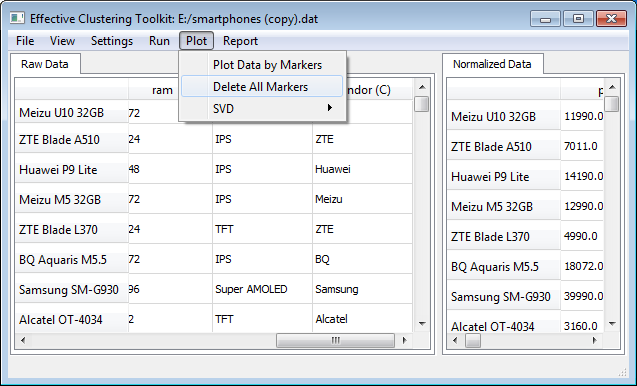
\includegraphics[width=0.65\textwidth]{img/deleteallmarkers}} \\
	
	\bottomrule
\end{tabularx}



\subsubsection{Построение SVD диаграммы}
\label{subsubsec:svd}
Для интегральной оценки структуры данных предусмотрена функция построения SVD диаграммы. Имеется возможность построения SVD диаграммы по нормализованным и не нормализованным данным.

\noindent\begin{tabularx}{\textwidth}{p{5.1cm}X}
	\toprule
	\textbf{Действие/Описание}& \textbf{Интерфейс}  \\
	
	\midrule
	\begin{titem}{Построить SVD диаграмму}
		Для построения SVD диаграммы в главном меню выбрать \menubox{\texttt{Plot}} $\Rightarrow$ \menubox{\texttt{SVD}} $\Rightarrow$ \menubox{\texttt{Normalized}} или \menubox{\texttt{Raw}} для построения диаграммы по нормализованным и не нормализованным данным соответственно.
	\end{titem}
	&  \raisebox{-\totalheight}{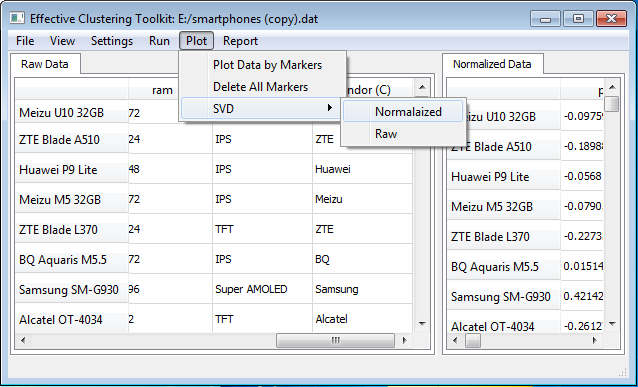
\includegraphics[width=0.65\textwidth]{img/svdplot}} \\
		
	\midrule
	\begin{titem}{Посмотреть результат}
		Построенная диаграмма откроется в новом окне.
	\end{titem}
	&  \raisebox{-\totalheight}{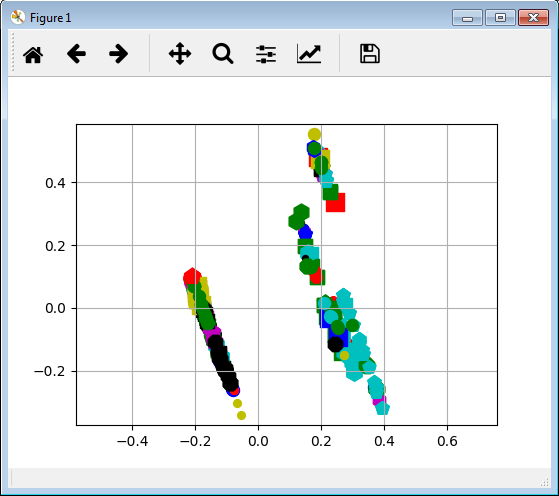
\includegraphics[width=0.65\textwidth]{img/svd}} \\
	
	\bottomrule
\end{tabularx}

\subsection{Генерация синтетических данных}
\label{subsec:generation}
Для генерирования искусственных данных необходимо вызвать диалог настройки параметры, указать все необходимые величины и сохранить сгенерированные данные в файл.

\noindent\begin{tabularx}{\textwidth}{p{5.1cm}X}
	\toprule
	\textbf{Действие/Описание}& \textbf{Интерфейс}  \\
	
	\midrule
	\begin{titem}{Открыть диалог генерации данных}
		Чтобы открыть диалог загрузки данных необходимо в главном меню программы выбрать \menubox{\texttt{File}} $\Rightarrow$ \menubox{\texttt{Data}} $\Rightarrow$ \menubox{\texttt{Generate}} 
	\end{titem}
	&  \raisebox{-\totalheight}{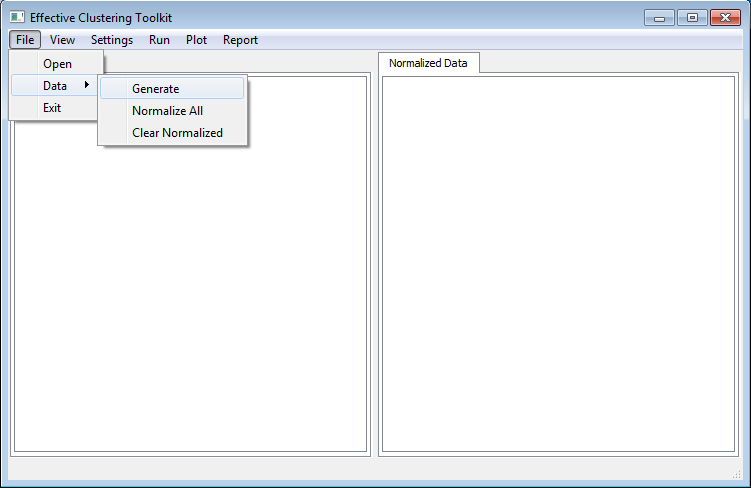
\includegraphics[trim={0 200 0 0},clip,width=0.65\textwidth]{img/generatemenu}} \\
	
	\midrule
	\begin{titem}{Указать параметры данных}
		В открывшемся диалоге необходимо указать параметры данных, по которым будет производиться генерация. Подробнее о параметрах генерации см. \cite{kovaleva}. В верхней части диалога отображается статическая информирующая диаграмма. Когда все параметры будут введены, нажать кнопку \menubox{\texttt{OK}} и в стандартном диалоге сохранения указать файл, в который требуется записать результат. 	
	\end{titem}
	&  \raisebox{-\totalheight}{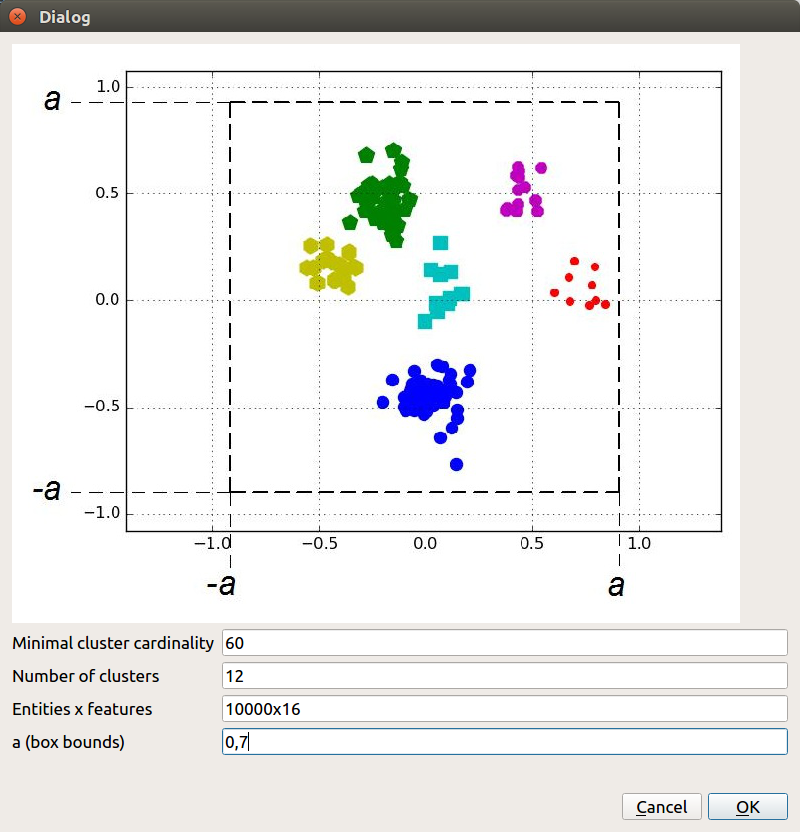
\includegraphics[width=0.65\textwidth]{img/generation.png}} \\
	
	\midrule
	\begin{titem}{Сохранить данные в файл}
	\end{titem}
	 & 	\parbox[t]{12cm}{ \vphantom{нечто} Сохранить данные в файл в стандартном файловом\\ диалоге.} \\

	\bottomrule
\end{tabularx}

\newpage
\subsection{Запуск кластеризации}

Для определения принадлежности объектов кластерам требуется установить параметры кластеризации и запустить алгоритм.

\noindent\begin{tabularx}{\textwidth}{p{5.1cm}X}
	\toprule
	\textbf{Действие/Описание}& \textbf{Интерфейс}  \\
	
	\midrule
	\begin{titem}{Открыть диалог выбора параметров}
		Пред запуском кластеризации потребуется задать общие параметры процедуры, по которым программа выберет конкретный алгоритм. Для этого необходимо из главного меню выбрать: \menubox{\texttt{Run}} $\Rightarrow$ \menubox{\texttt{Clustering}}. Подробнее про параметры см. \cite{amorim,kovaleva} и раздел \ref{sec:algs} После установки выбранных параметров для подтверждения нажать кнопку \menubox{\texttt{OK}}
	\end{titem}
	&  \raisebox{-\totalheight}{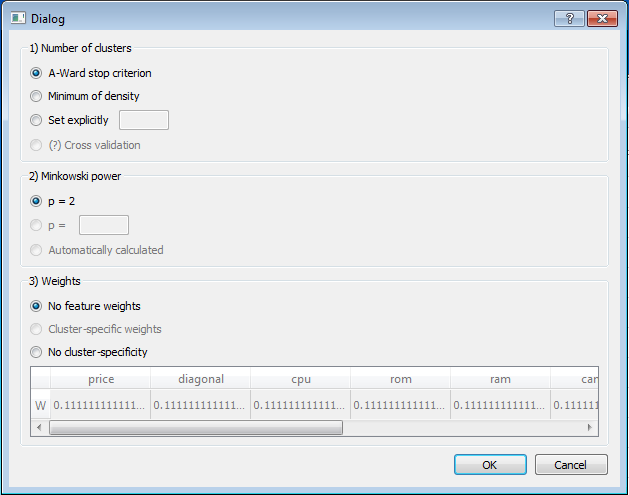
\includegraphics[width=0.65\textwidth]{img/runclusteringdialog.png}} \\
	
	\midrule
	\begin{titem}{Дождаться результатов кластеризации}	
		Сразу после нажатия кнопки \menubox{\texttt{OK}} начнется работа алгоритма кластеризации. Когда алгоритм закончит работу, появится окно, изображённое справа. Если в окне нажать кнопку \menubox{\texttt{Show Details}} то появится дополнительная информация о выбранном алгоритме и времени работы. Нажать кнопку  \menubox{\texttt{OK}}.
	\end{titem}
	&  \raisebox{-\totalheight}{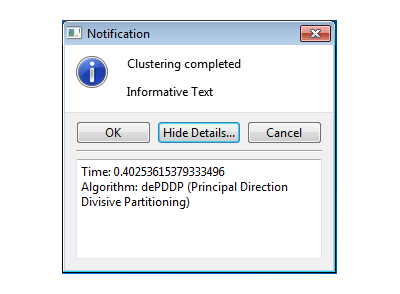
\includegraphics[width=0.65\textwidth]{img/resultinfo.png}} \\	
	
	\midrule
	\begin{titem}{Проверить заполнение столбца \texttt{Cluster\#}}
			В процессе кластеризации каждому объекту ставиться в соответствие номер кластера, которому он принадлежит. Для заданного объекта этот номер можно посмотреть в столбце ``\texttt{Cluster\#}''
	\end{titem}
	&  \raisebox{-\totalheight}{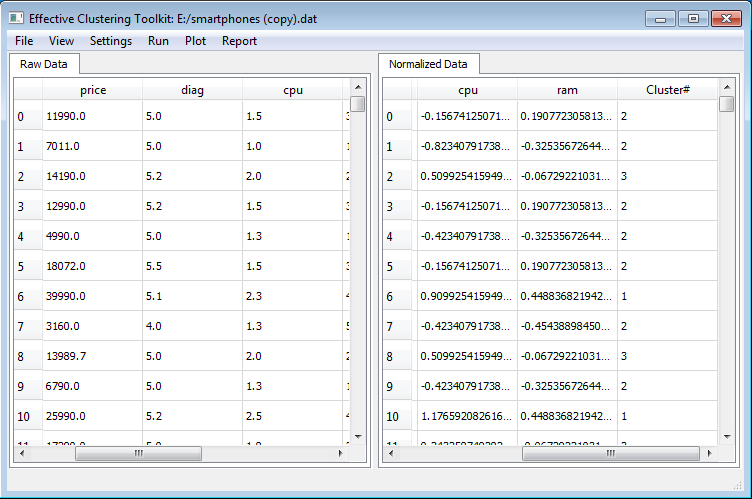
\includegraphics[width=0.65\textwidth]{img/clustercolumn}} \\	
	\bottomrule
\end{tabularx}

\subsection{Генерация отчёта}
\label{subsec:report}
Результаты кластеризации удобно анализировать по сгенерированному отчёту.

\noindent\begin{tabularx}{\textwidth}{p{5.1cm}X}
	\toprule
	\textbf{Действие/Описание}& \textbf{Интерфейс}  \\
	
	\midrule
	\begin{titem}{Сгенерировать отчёт}
		Для генерации отчёта в главном меню выбрать \menubox{\texttt{Report}} $\Rightarrow$ \menubox{\texttt{Show}}.
	\end{titem}
	&  \raisebox{-\totalheight}{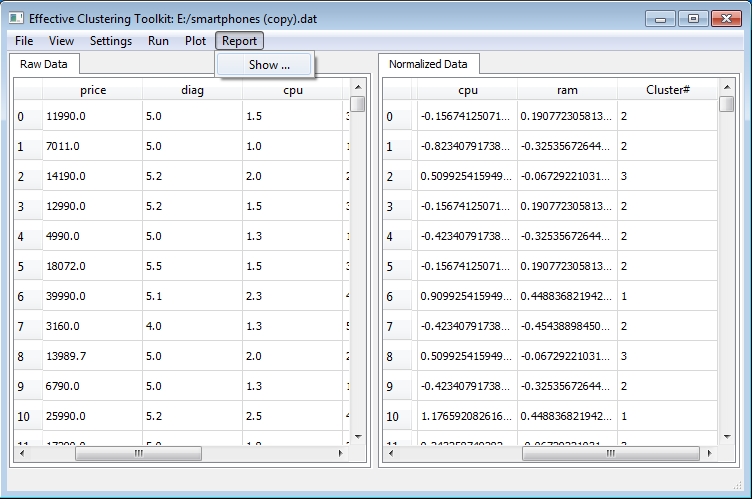
\includegraphics[width=0.65\textwidth]{img/showreport}} \\
	
	\midrule
	\begin{titem}{Посмотреть окно таблицы результатов}
		Отчёт состоит из двух окон. Первое --- окно с таблицей результатов. В этом окне приведена сводная таблица в которой строки соответствуют кластерам, а столбцы --- признакам. В ячейках указаны средние значения признака по кластеру. Красным цветом выделены ячейки, в которых относительная разность значения и средней величины признака по кластеру больше 30\%, соответственно синим --- меньше 30\%. Маржинальная строка содержит средние значения признаков по всем кластерам, а столбец --- число объектов в кластере.
	\end{titem}
	&  \raisebox{-\totalheight}{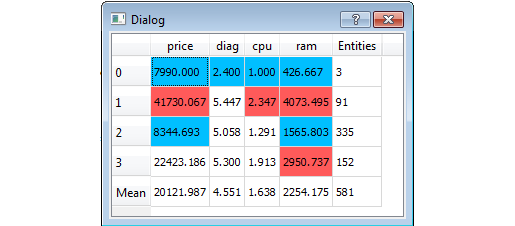
\includegraphics[width=0.65\textwidth]{img/reporttable}} \\
	
	\midrule
	\begin{titem}{Посмотреть окно текстового отчёта}
		Текстовый отчёт содержит все сведения относительно выбранного алгоритма, метода нормализации, и параметров каждого из кластеров.
	\end{titem}
	&  \raisebox{-\totalheight}{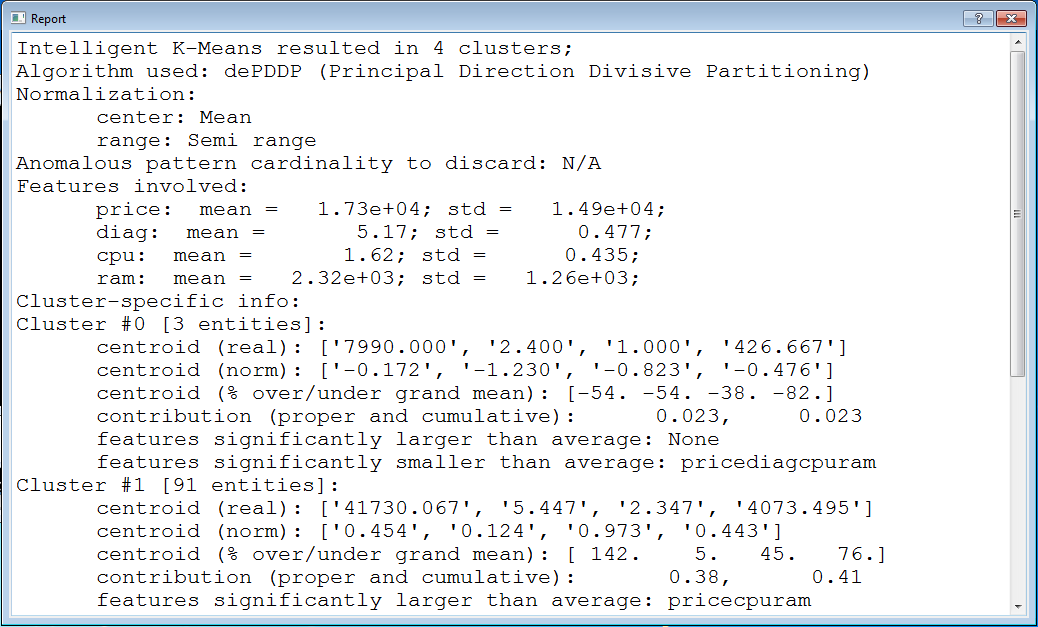
\includegraphics[width=0.65\textwidth]{img/reporttext}} \\
	
	\bottomrule
\end{tabularx}

\newpage
\subsection{Выход из программы}

\noindent\begin{tabularx}{\textwidth}{p{5.1cm}X}
	\toprule
	\textbf{Действие/Описание}& \textbf{Интерфейс}  \\
	
	\midrule
	\begin{titem}{Выйти из программы}
			Для выхода из программы в главном меню выбрать \menubox{\texttt{File}} $\Rightarrow$ \menubox{\texttt{Exit}}.
	\end{titem}
	&  \raisebox{-\totalheight}{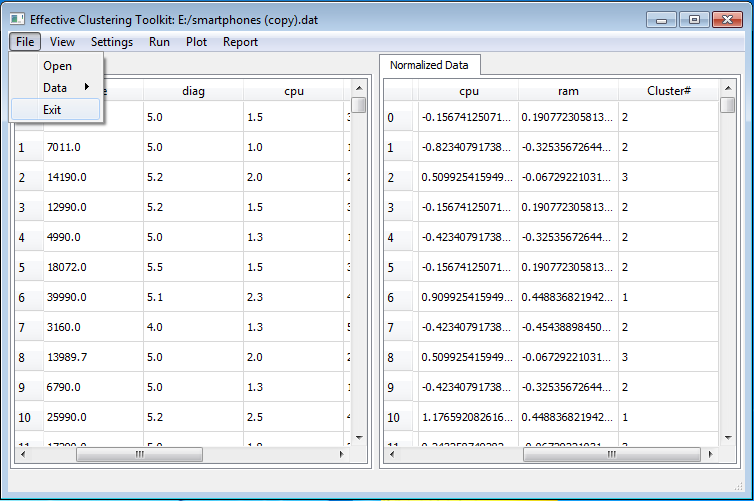
\includegraphics[width=0.65\textwidth]{img/exit}} \\
	
	\bottomrule
\end{tabularx}

\section{Алгоритмы кластеризации (краткое описание)}
\label{sec:algs}
\subsection{Алгоритм $ A-Ward $}
\label{subsec:a-ward}
Алгоритм A-Ward является усовершенствованием  широко известного алгоритма иерархической кластеризации Ward \cite{ward}. Этот алгоритм основан на пошаговом слиянии двух ближайших кластеров. На первом шаге все кластеры представлены в виде синглтонов, то есть кластеров, состоящих из единственного объекта, являющегося центроидом. Остановка алгоритма происходит при достижении числа кластеров, заданного пользователем. Для определения степени близости используется критерий, учитывающий число объектов в кластере и расстояние между центроидами.

Существенный недостаток алгоритма Ward --- его время работы. Для кластеризации большого числа объектов на начальных этапах работы требуется осуществить попарный перебор большого числа синглтонов. Авторы статьи \cite{amorim} предлагают устранить этот недостаток при помощи предварительного разбиения объектов. Предварительное разбиение используется как начальное состояние для работы Ward. В алгоритме Ward предлагается начинать рассмотрение с простейших кластеров, состоящих из единственного объекта, в то время как A-Ward использует кластеры, полученные при помощи метода аномальной кластеризации. 

Метод аномальной кластеризации находит и удаляет аномальные кластеры по одному, начиная со всего набора данных, до тех пор пока не останется объектов для рассмотрения. В основе этого метода лежит критерий k-means \cite{k-means}. Аномальным называется такой кластер, который наиболее удалён от центра данных. Центроид аномального кластера обновляется на каждом шаге, в то время как центр данных остаётся неизменным.

\subsection{Алгоритм $ A-Ward_{p\beta} $}
В реальных приложениях требуется анализировать зашумленные данные, включающие нерелевантные признаки. В этом случае оба алгоритма Ward и A-Ward проявляют себя как непригодные. Снизить влияние нерелевантных признаков позволяет введение весовых коэффициентов. В процессе работы алгоритма для каждого признака вычисляется вес, обратно пропорциональный разбросу признака внутри кластера.

Таким образом, алгоритм  A-Ward$_{p\beta} $ можно рассматривать как обобщение алгортма A-Ward. Основная идея обобщения состоит в том чтобы использовать метрику Минковского произвольной степени, а также назначить каждому признаку в пределах кластера определённый весовой коэффициент, учитывающий разброс этого признака внутри кластера. Параметры $ p $ и $ \beta $ являются степенями Минковского и весовых коэффициентов соответственно.

 Как и в случае с A-Ward, алгоритм A-Ward$_{p\beta} $ использует аномальную кластеризацию для предварительной ``разведки'' структуры данных и снижения времени работы, однако для алгоритма A-Ward$_{p\beta} $ аномальная кластеризация обобщена с учётом новых параметров.
 

\subsection{Алгоритм $ BiKM-R $}
	
Алгоритм bisecting k-means (раздвоение по методу k-средних) разбивает некоторый кластер $ S $ на два, при этом используя критерий минимума средних квадратов. Для инициализации алгоритма требуется указать начальные центроиды $ c_{1} $ и $ c_{2} $. На следующем этапе происходит альтернативная минимизация суммарной квадратичной ошибки, которая осуществляется за два шага. На первом шаге обновляется кластеры, то есть все объекты разделяются на те, которые расположены ближе к центроиду $ c_{1} $ (они образуют кластер $ S1 $ ) и те, которые ближе к $ c_{2} $ (кластер $ S2 $). На втором шаге для кластеров $ S1 $ и $ S2 $ вычисляются новые центориды $ c_{1}' $ и $ c_{2}' $. Процесс повторяется до тех пор пока происходят изменения центроидов кластеров. 

Результат алгоритма раздвоения может сильно зависеть от выбора исходных центроидов. Как правило, рекомендуется случайный выбор, но такое решение обеспечивает нестабильный результат. Как и в случае с агломеративным алгоритмами, метод аномальных кластеров может быть использован для предварительного выявления центроидов рациональным образом.  В такой постановке для инициализации алгоритма раздвоения используются центроиды двух наибольших аномальных кластеров. 

Для остановки алгоритма авторами статьи \cite{kovaleva} предложен новый критерий, основанный на проецировании точек кластеров на произвольные направления. Пусть на некотором этапе работы алгоритма имеется $ S_{k} $ кластеров. Первым шагом генерируются $ s $ случайных векторов $ p_{i},\:i=1,...,s $. Для генерации используется нормальное сферическое распределение со средним в начале координат и $ \sigma^{2}=\dfrac{1}{V} $ , где $ V $ – количество признаков. На втором шаге каждый элемент $ x $ каждого кластера $ S_{k}\:(k=1,...,K) $  проецируется на направления $ p_{i} $, координаты проекции определяются как скалярное произведение: $ x_{t}=<x,p_{t}> $ . Для каждого направления вычисляется функция плотности $ f_{k}^{t} $ по методу ядерной оценки. Если для некоторого кластера $ k $ отношение $ \epsilon_{k} $ числа направлений, для которых функции плотности  $ f_{k}^{t} $ имеют по крайне мере один минимум к общему числу направлений меньше заданного пользователем порога $ \epsilon $ , то кластер $ k $ не разбивается. Для разделения выбирается в первую очередь кластер с наибольшим отношением $ \epsilon_{k}/\epsilon $ . Выбранный кластер разбивается но наиболее глубокому минимуму.  

\subsection{Алгоритм $ dePDDP $}

Алгоритм dePDDP (Principal Direction Divisive Partitioning) относится к иерархическим дивизивным и является модифицированной версией алгоритма PDDP \cite{PDDP} . Изначально критерий разделения кластера на две части был относительно простым: предлагалось разделить кластер по главной компоненте на положительную и отрицательную части. Впоследствии эта идея была усовершенствована при помощи правила, учитывающего распределение данных \cite{tas}. Разбиение производится по наиболее глубокому минимуму функции плотности данных, спроецированных на первую главную компоненту. Это правило примечательно тем, что может быть использовано для разрешения двух сопряженных проблем: выбора кластера для разбиения и остановки алгоритма. Для разбиения выбирается кластер с наименьшим минимумом среди всех терминальных кластеров. Если кластер имеет монотонную или выпуклую функцию плотности, то такой кластер не может быть разделен по критерию данного алгоритма. Экспериментально было показано, что алгоритм, работающий на описанных принципах эффективно решает задачу кластеризации как на реальных данных, так и на синтетических. 
Оценка функции плотности осуществляется по методу ядерной оценки.


\section{Примеры работы с программой}
\subsection{Нормализация}
\subsubsection{Нормализация с центрированием по среднему и масштабированием по полуразмаху}
\label{subsubseq:example_norm1}

В данном разделе рассматривается пример нормализации признаков обучающего файла \texttt{smartphones.dat} с центрированием по среднему и масштабированием по полуразмаху. 

\noindent\begin{tabularx}{\textwidth}{p{5.1cm}X}
	\toprule
	\textbf{Действие/Описание}& \textbf{Интерфейс}  \\
	\toprule
	
	\begin{titem}{Запустить бинарный файл программы}
		Дважды нажать левой кнопкой мыши (ЛКМ) на значке \texttt{INDACT.exe} 
	\end{titem}
	&  \raisebox{-\totalheight}{\includegraphics[width=0.65\textwidth]{img/runexe}} \\
	
	\midrule
	\begin{titem}{Открыть диалог загрузки файла}
			Последовательно нажать в главном меню пункты \menubox{\texttt{File}} $ \Rightarrow $ \menubox{\texttt{Open}}.
	\end{titem}
	&  \raisebox{-\totalheight}{\includegraphics[trim={0 200 172 0 0},clip,width=0.65\textwidth]{img/fileopen}} \\
	
	\midrule
	\begin{titem}{Выбрать текстовый файл с данными}
		В файловом диалоге выбрать загружаемый файл \texttt{INDACT/example/} \texttt{smartphones.dat} и нажать кнопку \menubox{\texttt{Open}}.  
	\end{titem}
	&  \raisebox{-\totalheight}{\includegraphics[width=0.65\textwidth]{img/filedialog.png}} \\	
	
	\midrule
	\begin{titem}{Убедиться что файл загружен}
		Посмотреть, что вкладка ``\texttt{Raw Data}'' заполнилась данными из файла.
	\end{titem}
	&  \raisebox{-\totalheight}{\includegraphics[width=0.65\textwidth]{img/loadeddata.png}} \\
	
	\midrule
	\begin{titem}{Установить признак \texttt{name} как индекс}		
		Отрыть контекстное меню ПКМ и выбрать \menubox{\texttt{Set}} $\Rightarrow$ \menubox{\texttt{As Index}}  
	\end{titem}
	&  \raisebox{-\totalheight}{\includegraphics[width=0.65\textwidth]{img/asindex}} \\
	
	\midrule
	\begin{titem}{Убедиться что признак выставился}
		Результат выполнения предыдущей операции показан на рисунке справа. Теперь числовые индексы заменены названиями телефонов. 
	\end{titem}
	&  \raisebox{-\totalheight}{\includegraphics[width=0.65\textwidth]{img/asindexcompleted.png}} \\
	
	\midrule
	\begin{titem}{Удалить признак \texttt{vendor}}		
		Вызвать контекстное меню на признаке \texttt{vendor} при помощи ПКМ и выбрать пункт \menubox{\texttt{Delete}}.
	\end{titem}
	&  \raisebox{-\totalheight}{\includegraphics[width=0.65\textwidth]{img/deletevendor.png}} \\
	
	\midrule
	\begin{titem}{Убедиться что признак удалён}
		Результат удаления признака \texttt{vendor} показан на рисунке справа. Видно, что признак \texttt{vendor} больше не отображается во вкладке ``\texttt{Raw Data}'' 
	\end{titem}
	&  \raisebox{-\totalheight}{\includegraphics[width=0.65\textwidth]{img/deletevendorresult.png}} \\
	
	\midrule
	\begin{titem}{Открыть окно нормализации}
		Выбрать в главном меню пункты \menubox{\texttt{Settings}} $ \Rightarrow $ \menubox{\texttt{Normalization}}.
	\end{titem}
	&  \raisebox{-\totalheight}{\includegraphics[width=0.65\textwidth]{img/opennormalizationdialogexample}} \\
	
	\midrule
	\begin{titem}{Выставить параметры нормализации}
		Выставить параметры нормализации как показано на рисунке справа. Переключатель ``\texttt{Normalization disabled}'' должен быть снят, значение \texttt{Center} выбрано \texttt{Mean}, а значение \texttt{Range} --- \texttt{Semi range}. Подтвердить ввод, нажав \menubox{\texttt{OK}}. 
	\end{titem}
	&  \raisebox{-\totalheight}{\includegraphics[width=0.65\textwidth]{img/normmeansemirange}} \\

	\midrule	
	\begin{titem}{Запустить нормализацию всех признаков }
		Для запуска нормализации всех признаков сразу, требуется в главном меню выбрать \menubox{\texttt{File}} $ \Rightarrow $ \menubox{\texttt{Data}}  $ \Rightarrow $  \menubox{\texttt{Normalize All}}.
	\end{titem}
	&  \raisebox{-\totalheight}{\includegraphics[width=0.65\textwidth]{img/normalizeallexample}} \\	
	
	\midrule
	\begin{titem}{Подтвердить нормализацию категориального признака}
		Так как данные включают в себя категориальный признак \texttt{stype}, то программа запросит подтверждение разложения признака по количеству уникальных значений. Нажать кнопку \menubox{\texttt{OK}}.
	\end{titem}
	&  \raisebox{-\totalheight}{\includegraphics[width=0.65\textwidth]{img/approvenominalexample}} \\
	
	\midrule
	\begin{titem}{Посмотреть результат}
		После нормализации признаков результат будет отображен во вкладке ``\texttt{Normalized Data}''
	\end{titem}
	&  \raisebox{-\totalheight}{\includegraphics[width=0.65\textwidth]{img/normalizeallresultexample}} \\
	
	\bottomrule
\end{tabularx}

\subsubsection{Нормализация с центрированием по Минковскому и масштабированием по стандартному отклонению}
\label{subsubseq:example_norm2}
Теперь рассмотрим пример нормализации данных из демонстрационного примера с центрированием Минковского.

\noindent\begin{tabularx}{\textwidth}{p{5.1cm}X}
	\toprule
	\textbf{Действие/Описание}& \textbf{Интерфейс}  \\
	\toprule
	
	\begin{titem}{Запустить программу и загрузить файл}
	\end{titem}
	& 	\parbox[t]{12cm}{ \vphantom{нечто} Выполнить пункты 1--9 из предыдущего примера (\ref{subsubseq:example_norm1}).} \\
	
	\midrule
	\begin{titem}{Выставить параметры нормализации}
		Выставить параметры нормализации как показано на рисунке справа. Переключатель ``\texttt{Normalization disabled}'' должен быть снят, значение Center выбрано \texttt{Minkowski Center}, величина \texttt{Minkowski Power} выставлена равной \texttt{1.5}, а параметр \texttt{Range} выбран \texttt{Standard deviation}.
	\end{titem}
	&  \raisebox{-\totalheight}{\includegraphics[width=0.65\textwidth]{img/normminkowski}} \\
	
	\midrule
	\begin{titem}{Нормализовать все признаки}
	\end{titem}
	& 	\parbox[t]{12cm}{ \vphantom{нечто} Выполнить пункты 11--12 из предыдущего примера (\ref{subsubseq:example_norm1}).} \\
	
	\midrule
	\begin{titem}{Посмотреть результат}
		После нормализации признаков результат будет отображён во вкладке ``\texttt{Normalized Data}''
	\end{titem}
	&  \raisebox{-\totalheight}{\includegraphics[width=0.65\textwidth]{img/normalizeallresultexamplemink}} \\
	
	\bottomrule	
\end{tabularx}


\subsection{Кластеризация}
\subsubsection{Кластеризация с автоматическим выбором числа кластеров}
\label{subsubsec:clustering_example1}
Рассмотрим пример кластеризации с использованием метода, который предусматривает автоматическое вычисление числа кластеров в процессе работы. Используем для этого процедуру нормализации проиллюстрированную ранее. Выберем типичные значения параметров нормализации: центрирование по среднему, масштабирование полуразмахом (см. \ref{subsubseq:example_norm1}). 


\noindent\begin{tabularx}{\textwidth}{p{5.1cm}X}
	\toprule
	\textbf{Действие/Описание}& \textbf{Интерфейс}  \\
	\toprule
	
	\begin{titem}{Запустить программу, загрузить файл и нормализовать признаки}
		Выполнить все пункты из первого примера(\ref{subsubseq:example_norm1}). Для кластеризации требуются нормализованные признаки.
	\end{titem}
	& \raisebox{-\totalheight}{\includegraphics[width=0.65\textwidth]{img/normalizeallresultexample}} \\
	
	\midrule
	\begin{titem}{Открыть окно кластеризации}
		Пред запуском кластеризации потребуется задать общие параметры процедуры, по которым программа выберет конкретный алгоритм. Для этого необходимо из главного меню выбрать: \menubox{\texttt{Run}} $\Rightarrow$ \menubox{\texttt{Clustering}}. 
	\end{titem}
	&  \raisebox{-\totalheight}{\includegraphics[width=0.65\textwidth]{img/runclusteringexample1}} \\
	
	\midrule
	\begin{titem}{Установить параметры алгоритма кластеризации}
		Установить параметры кластеризации как показано на рисунке справа. В группе регулирующей число кластеров установить переключатель \texttt{Minimum of density} для выбора числа кластеров по минимуму функции плотности. Степень Минковского установить равной 2, отметив соответствующий переключатель. Веса признаков в данном примере не используются. Нажать \menubox{\texttt{OK}}. 
	\end{titem}
	&  \raisebox{-\totalheight}{\includegraphics[width=0.65\textwidth]{img/clusteringdialogexample1.png}} \\
	
	\midrule
	\begin{titem}{Дождаться завершения кластеризации}
		Когда алгоритм закончит работу, появится окно, изображённое справа. Если в окне нажать кнопку \menubox{\texttt{Show Details}} то появится дополнительная информация о выбранном алгоритме и времени работы. Нажать кнопку  \menubox{\texttt{OK}}.
	\end{titem}
	 &  \raisebox{-\totalheight}{\includegraphics[width=0.65\textwidth]{img/resultinfo.png}} \\		
	
	\midrule
	\begin{titem}{Посмотреть кластерную принадлежность}
		После завершения кластеризации во вкладке ``\texttt{Normalized Data}'' будет заполнен столбец \texttt{Cluster\#} как показано на рисунке справа.	
	\end{titem}
	&  \raisebox{-\totalheight}{\includegraphics[width=0.65\textwidth]{img/clustercolumnexample1}} \\		
	
	
	\midrule
	\begin{titem}{Сгенерировать отчёт}
		Для генерации отчёта в главном меню выбрать \menubox{\texttt{Report}} $\Rightarrow$ \menubox{\texttt{Show}} (см. \ref{subsec:report}).	
	\end{titem}
	&  \raisebox{-\totalheight}{\includegraphics[width=0.65\textwidth]{img/generatereportclusteringexample1}} \\		
	
	\midrule
	\begin{titem}{Посмотреть отчёт}
		Вид отчёта показан на рисунке справа. Сверху показана таблица интегрального представления, а снизу --- текстовый отчёт.  
	\end{titem}
	&  \raisebox{-\totalheight}{\includegraphics[width=0.65\textwidth]{img/reporttableclusteringexample1}}
	
	\raisebox{-\totalheight}{\includegraphics[width=0.65\textwidth]{img/textreportclusteringexample2}} \\	
	
	
	\bottomrule
\end{tabularx}

\newpage
\subsubsection{Кластеризация с явно заданным числом кластеров}

Если известно конкретное число кластеров входящих в состав данных, можно применить методы, подразумевающие явный ввод с клавиатуры. Например, число кластеров позволяет задать метод A-Ward (см. раздел \ref{subsec:a-ward}).

\noindent\begin{tabularx}{\textwidth}{p{5.1cm}X}
	\toprule
	\textbf{Действие/Описание}& \textbf{Интерфейс}  \\
	\toprule
	
	\begin{titem}{Запустить программу, загрузить файл и нормализовать признаки}
		Выполнить все пункты из второго примера (\ref{subsubseq:example_norm2}). Для кластеризации требуются нормализованные признаки. Для данного примера используется нормализация с центрированием Минковского.
	\end{titem}
	& \raisebox{-\totalheight}{\includegraphics[width=0.65\textwidth]{img/normalizeallresultexamplemink}} \\
	
	\midrule
	\begin{titem}{Открыть окно кластеризации}
		Пред запуском кластеризации потребуется задать общие параметры процедуры, по которым программа выберет конкретный алгоритм. Для этого необходимо из главного меню выбрать: \menubox{\texttt{Run}} $\Rightarrow$ \menubox{\texttt{Clustering}}. 
	\end{titem}
	&  \raisebox{-\totalheight}{\includegraphics[width=0.65\textwidth]{img/runclusteringexample1}} \\
	
	\midrule
	\begin{titem}{Установить параметры алгоритма кластеризации}
		Установить параметры кластеризации как показано на рисунке справа. В группе регулирующей число кластеров установить переключатель \texttt{Set explicitly} для ввода числа кластеров с клавиатуры. Ввести число кластеров 10. Степень Минковского установить равной 1.5, отметив переключатель \texttt{p=}. Для назначения кластер-специфичных весов выбрать переключатель \texttt{Cluster-specific weights} (см. \cite{amorim}). Нажать \menubox{\texttt{OK}}. 
	\end{titem}
	&  \raisebox{-\totalheight}{\includegraphics[width=0.65\textwidth]{img/clusteringdialogexample2}} \\
	
	\midrule
	\begin{titem}{Дождаться завершения кластеризации}
		Когда алгоритм закончит работу, появится окно, изображённое справа. Если в окне нажать кнопку \menubox{\texttt{Show Details}} то появится дополнительная информация о выбранном алгоритме и времени работы. Нажать кнопку  \menubox{\texttt{OK}}.
	\end{titem}
	& \raisebox{-\totalheight}{\includegraphics[width=0.65\textwidth]{img/clusteringfinishedexample2}} \\		
	
	\midrule
	\begin{titem}{Посмотреть кластерную принадлежность}
		После завершения кластеризации во вкладке ``\texttt{Normalized Data}'' будет заполнен столбец \texttt{Cluster\#} как показано на рисунке справа.	
	\end{titem}
	&  \raisebox{-\totalheight}{\includegraphics[width=0.65\textwidth]{img/clustercolumnexample2}} \\		
	
	\midrule
	\begin{titem}{Сгенерировать отчёт}
		Для генерации отчёта в главном меню выбрать \menubox{\texttt{Report}} $\Rightarrow$ \menubox{\texttt{Show}} (см. \ref{subsec:report}).	
	\end{titem}
	&  \raisebox{-\totalheight}{\includegraphics[width=0.65\textwidth]{img/generatereportclusteringexample2}} \\		
	
	\midrule
	\begin{titem}{Посмотреть отчёт}
		Вид отчёта показан на рисунке справа. Сверху показана таблица интегрального представления, а снизу --- текстовый отчёт. Как видно из интегрального отчёта, некоторые кластеры не представительны, поэтому в реальных условиях, возможно, следовало бы рассмотреть другие значения параметров. 
	\end{titem}
	&  \raisebox{-\totalheight}{\includegraphics[width=0.65\textwidth]{img/reporttableclusteringexample2}}
	
	\raisebox{-\totalheight}{\includegraphics[width=0.65\textwidth]{img/textreportclusteringexample2}} \\	

\bottomrule
\end{tabularx}

% glossary
%\renewcommand{\glossaryname}{\centerline{\MakeUppercase{Словарь терминов (добавить примеры)}}}

%\clearpage
\setlist[description]{leftmargin=!, labelwidth=-0.5em} % Change for glossaries
\glsaddall

\addcontentsline{toc}{section}{Аббревиатуры}
\printglossary[type=\acronymtype,nonumberlist,style=acrostyle]

\newpage
\addcontentsline{toc}{section}{Словарь терминов}
\printglossary[nonumberlist]
\setlist[description]{style=standard} % reset settings back to default

\newpage
\nocite{amorim} \nocite{ward} \nocite{boley} \nocite{tasoulis} \nocite{kovaleva} \nocite{mirkin}
\addcontentsline{toc}{section}{Список литературы}
\bibliography{bibliography}

\end{document} 
